\chapter{Objectifying Jazz Harmony}

%Gjerdingen's bias complaint
In his recent work, Robert Gjerdingen summarizes the process of musical corpus analysis and issues a warning to its practitioners:\footnote{\cite{gjerdingen2014}, p.\ 193.}
\begin{quote}
``A simple recipe for doing a corpus study of any type
might read as follows:
\begin{enumerate}
	\item Define the set of elements believed to occur within
the corpus.
	\item Calculate appropriate statistics on the time series of
those elements.
	\item From those statistics, deduce pertinent norms or
rules for the corpus.
\end{enumerate}
While stages 2 and 3 may be amenable to numerical
methods and explicit algorithms, stage 1 may not. It is
thus often at stage 1 that the researcher makes decisions
that reveal a presentist or historicist bias."
\end{quote}

As Gjerdingen rightly notes, analysts often -- or perhaps \emph{must} -- make choices about the nature of the objects and processes under study well outside the frame of data-driven or statistical testing.\footnote{Recall, for example, Chapter 1's description of non-recursive roman numeral studies (\cite{tymoczko2010local}) hierarchical phrase parsing (\cite{rohrmeier2007}), and generative blues progressions (\cite{steedman1984}), each of which requires object assumptions to get off the ground.}  In the context of jazz, a researcher might produce a statistical model of chord-to-chord jazz progressions which is admirably agnostic about the types of progressions likely to result -- but which assumes as a starting point that chords have very particular properties arising from the history of music theory and the affordances of printed or digitized scores.  If the objects of harmonic importance are assumed to be consonant, tertian stacks, with unambiguous roots in the bass, whose notes sound at precisely the same moment, and which might be decorated with a variety of comparatively-unimportant embellishing tones, an analyst can generate certain kinds of statistics describing their behavior.  There is no guarantee, or at least no empirical guarantee, that the resulting statistical picture reflects categories particularly relevant to the corpus at hand.  If analysts are not to allow statistical methods to shoehorn particular data into pre-chosen categories, we must provide ways of specifying and generating categories of chord object from the data in as transparent a way as possible.

To bring chord categories into the light of day, I propose representations connecting observable pitch features to chord objects to which they might be seen to refer in productive ways.  Starting from chord definitions similar to those found in the jazz theory literature, I consider both voicings and scale-degree sets as potential categories permitting communication between algorithmic statistics and human interpreters.  Two productive results ensue.  First, I show that it is possible to re-create many of the chord categories currently employed with a minimum number of prior assumptions; second, I isolate harmonic objects for syntactic study in later chapters.  In this way, I mean the title of this chapter in a very literal sense: what follows is a discussion of how to make at least two kinds of objects out of jazz performance data.

%Corpus analysis + Kockelmanian semiotics can unpack and potentially avoid this problem
Gjerdingen's step (1) above implicitly questions ontological assumptions regarding harmonic processes, and as I unpack some of its implications for jazz syntax, I will frame the complicated relationship between harmonic objects and the selection and representation of their indices in semiotic ontological terms taken from linguistic anthropologist Paul Kockelman.\footnote{I refer especially to \cite{kockelman2013} and \cite{kockelman2013anthropology}.  For a formal introduction to the relevant models, see the former; for an example of their application, see the latter.} The abstract terminology and unusual ontology that result arise as both a consequence and motivation.  My concern is to produce as clear an \emph{epistemic} pathway as possible and to see what ontological structure results.  Rather than starting with traditional assumptions about chords, scales, and non-harmonic tones, and then trying to find a pathway to connect those abstractions to musical surfaces or analyses, I want to align a jazz harmonic ontology with a corpus statistical epistemology as closely as possible.  Doing so may require re-configuring traditional ontological assumptions about harmony (jazz or otherwise).

\section{Voicing Seventh Chords}
%Introduce seventh chords as ``fundamental"
Jazz theory manuals tend to emphasize a tripartite typology of chord types, where the basis of most jazz chords can be described in terms of seventh chords in a way analogous to traditional triadic descriptions of western art music.  As Henry Martin notes,
\begin{quote}
``Triads are not necessarily normative.  In fact, they are relatively rare in some styles where three types of seventh chords are the most common harmonic entities (major-seventh, minor-seventh, and dominant-seventh)."\footnote{\cite{martin1980}, p.\ 7.  Martin's dissertation is the most sustained, serious treatment of strict quality-centric chord category formation I have seen in the jazz literature.  For similar typological claims, see \cite{mehegan1959} and \cite{levine1989}.}
\end{quote}
As soon as Martin postulates these objects, he specifies that their traces in actual performance have particular properties: ``The perfect fifths within many jazz chords," Martin explains, ``are often unnecessary for the specification of harmonic type."\footnote{\cite{martin1980}}  Rather, the root, third, and seventh are assumed to be the primary determiners of chord identity.  An imagined jazz performer starts from a sequence of chord symbols, envisions these crucial members of each chord, and then chooses additional notes to fill out or embellish each sonority.

Most jazz manuals move on to offer nuanced advice regarding what notes to add.  Mark Levine's ``chart of the \emph{possible} notes that you can add to three-note minor seventh, dominant seventh, and major seventh voicings," shown in Figure~\ref{levineextensions}, is typical of the genre.\footnote{The quote and chart both come from \cite{levine1989}, p.\ 33.}
\begin{figure}
	\caption{Mark Levine's chart of possible additions to the common three-note seventh chord voicings.}
	\label{levineextensions}
	\centering
	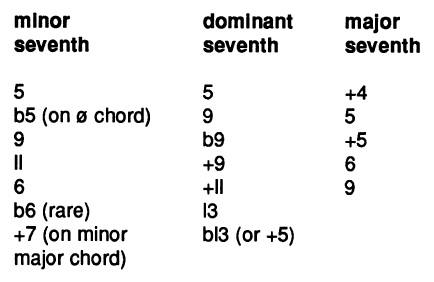
\includegraphics[width=3.1in]{levineextensions.jpg}
\end{figure}
There are a variety of ways through which it might be possible connect this simple model to jazz performance data.  Translated into corpus-analytic language, these traditional chord-quality voicing rules can be tested against the data of the Yale Jazz MIDI Piano (YJaMP) corpus.  An algorithm may look for root-third-seventh voicings (with various added tones) as signs standing for the seventh chords Martin places at the bedrock of jazz syntax.

In the presence of possible added tones, root determinations may be ambiguous or impossible to automate (or even hand-annotate consistently).  To sidestep this issue, I ask a simpler but analogous question: what chords occur in the YJaMP corpus which contain the three identifying chord tones listed above voiced in root-third-seventh ascending register within an octave?  For example, using a labeling system in which voicings are described by their semitonal distances above the bass note, what kinds of voicings contain $[0,4,10]$?

\begin{table}
\caption{Frequently-occurring corpus slices including $[0,4,10]$ voicing subsets.  These primarily include traditional dominant seventh chords with various added tones.  Note the traditionally unexpected appearance of $[0,4,10,17]$.  On what basis do we teach students to ``avoid" this natural 11?  What is its nature?}
  \centering
\begin{tabular}{l | l | l}
\hline\hline
Voicing & Counts & Additions \\ [0.5ex]
\hline
$[0, 4, 10]$ & 358 &  \\ 
$[0, 4, 10, 19]$ & 62 & add \nth{5} \\ 
$[0, 4, 10, 22]$ & 52 & double \nth{7} \\ 
$[0, 4, 10, 15]$ & 42 & $\sharp$\nth{9} \\ 
$[0,4,10,16]$ & 41 & double \nth{3} \\ 
$[0,2,6,12]$ & 40 & double \nth{7} \\ 
$[0,4,7,10]$ & 36 & add \nth{5} \\ 
$[0,4,10,21]$ & 36 & add \nth{13} \\ 
$[0,4,10,14]$ & 30 & add \nth{9} \\ 
$[0,4,10,13]$ & 29 & add $\flat$\nth{9} \\ 
$[0,4,10,17]$ & 23 & add \nth{11} \\ 
$[0,4,10,20]$ & 21 & add $\sharp$\nth{5} \\ 
$[0,4,10,18]$ & 21 & add $\sharp$\nth{11} \\ 
$[0,4,10,26]$ & 20 & add \nth{9} \\ 
$[0,4,10,28]$ & 20 & double \nth{3} \\[1ex]
\hline
\end{tabular}
\label{[0,4,10]}
\end{table}

Table~\ref{[0,4,10]} lists the most frequent voicings with dominant-seventh subsets.  To minimize reductive assumptions about non-harmonic tones, I search through ``salami slices" advocated by White and Quinn, verticalities generated from a na\"{i}ve approach agnostic about which pitches in a given stack should or can be disregarded.\footnote{For a full treatment of salami slice ideology, see \cite{wq2017}.}  As an algorithm thinly ``slices" the YJaMP performance corpus, it tracks each appearance and disappearance of a pitch, treating each resulting verticality as a potential chord, regardless of its pitch content.\footnote{White and Quinn trace their use of salami slices to comments by Ligeti; see \cite{wq2017}.} The most frequent chord additions match recommendations like those of Figure~\ref{levineextensions} almost precisely: chord tones like root, third, fifth, and seventh are added or doubled; diatonic extensions like 9 and 13 are added; alterations like $\sharp 9$, $\flat 9$, $\sharp 5$, and $\sharp 11$ are common.  The only place where the table of common voicings appears to disagree with received wisdom is in the frequent appearance of $[0,4,10,17]$, an apparent natural 11 chord.  What is the status of this observed sonority?

Levine, among many others, advocates against the ontological primacy of such sonorities.  Giving an explicit reason to discount this ``unusual" chord (but frequent slice) requires a kind of two-step ideological appeal to reduction like the following:
\begin{enumerate}
	\item This chord contains a dissonant or quality-ambiguating minor 9th between its third and eleventh, rendering it problematic and giving it some kind of unstable acoustical status.
	\item The chord cannot fulfill its usual harmonic function as is: instead, it likely functions as some kind of passing or neighboring chord in the context of a less-problematic, more-normative dominant sonority.
\end{enumerate}
A corpus-supported analog to step (1) is unclear, and it would likely fall prey to Gjerdingen's analyst-bias objections.  Claims of problematic consonance and dissonance would require psycho-acoustical modeling, appealing to measurable properties of sounded chords and human responses to them.  Such studies are more common in the classical literature, but some jazz work in this direction has begun to appear.\footnote{The auditory perception foundations of this kind of work stretch back to \cite{helmholtz1863}.  For an overview of sound  and critical band hearing research from the first half of the twentieth century, see \cite{scharf1961}; the later work of Plomp and Levelt aims this apparatus toward tonal consonance (see \cite{plomp1965}).  \cite{longuet1979} is emblematic of the turn taken when computational resources meet acoustics in a musical context, while a thorough treatment of modern psychoacoustics in common-practice classical music theory can be found in \cite{parncutt2012}.  \cite{mcgowan2008} engages with Helmholtzian perception in the context of jazz consonance and dissonance, but it draws on few of the empirical or computational tools of the above sources.}  Any corpus analytical claim regarding the impact of acoustical consonance on chord usage, if not accompanied by psycho-acoustical justification, would encode the analyst's expectations regarding jazz syntax into the data selection process, biasing any results meant to indicate how voicings appear in the corpus.  Pitch-based corpus statistics regarding which voicings are most common or important cannot be filtered for psycho-acoustic properties without biasing the results toward the whatever preconceptions the analyst chooses to encode.

A corpus of performances can be made to suggest lines of reasoning like (2); a tally of what kinds of voicings tend to follow $[0,4,10,17]$ provides a cursory suggestion as to its use.  If this voicing tends to progress to subsequent harmonies in a way strongly similar to (or different from) other dominant voicings, it may (or may not) stand in for Martin's dominant seventh chord category, despite Levine's intervallic contraindications.

Figure~\ref{[0,4,10,17]} shows the most common voicing salami slices to appear within 50 slices of $[0,4,10,17]$.\footnote{Note that this flexible span reflects the appearance or disappearance of any single note 50 consecutive times.  At extremely quick tempos or during fast runs, 50 slices could pass in a couple of seconds; at slow tempos or during moments of stasis, the same number of slices might cover tens of seconds (or, formally, an arbitrarily long time).}  Each destination slice is indexed here by both its semitonal voicing structure and the number of semitones its bass lies above or below the bass note of $[0,4,10,17]$.  For example, the most common nearby destination slice is the voicing $[0,1,5]$, the seventh, root, and third of a major-seventh chord in registrally-ascending order (see the yellow line in Figure~\ref{[0,4,10,17]}). The seventh of this destination chord (found in the bass) lies a major third above the bass of the preceding $[0,4,10,17]$ chord (hence the initial 4-semitone entry in the relevant parenthesis).  While the slice counting algorithm has made no assumptions of any kind about key, this ``progression" implies traditional root motion down by fifth, indicating that $[0,4,10,17]$ most frequently appears in the context of dominant-tonic motion.  Crucially, this dominant-tonic motion typically occurs on a time scale of many (18-30) slices; during that span, the ``unusual" voicing has plenty of opportunities to ``resolve" or clarify its status: melodic motion might connect it to a more normative dominant-seventh, like $[0,4,10,14]$, or a consonant dominant triad, like $[0,16,19]$ (see the blue line in Figure~\ref{[0,4,10,17]}).  Due to the wide variety of destination voicings found after $[0,4,10,17]$, this is comparatively weak support for the two-step reduction outlined above, but it does indicate the form such an appeal might take in corpus analytic terms.  An analysis based solely on voicing structure produces an observation defying the properties of the voicing model, so the analyst turns to some behavioralist reduction criteria to normalize the results.

\begin{figure}
	\caption{Following slice behavior for $[0,4,10,17]$ voicings.  The voicing appears most frequently in the neighborhood of $[0,1,5]$ voicings a major third up (yellow line), implying its participation in $V^7 \rightarrow I^2$ dominant-tonic progressions.  But salami slice adjacencies also imply intra-syntactic progressions at shorter scales; the blue line plots the appearance of $[0,16,19]$, the dominant triad sharing a bass note and root with the preceding $[0,4,10,17]$.}
	\label{[0,4,10,17]}
	\centering
	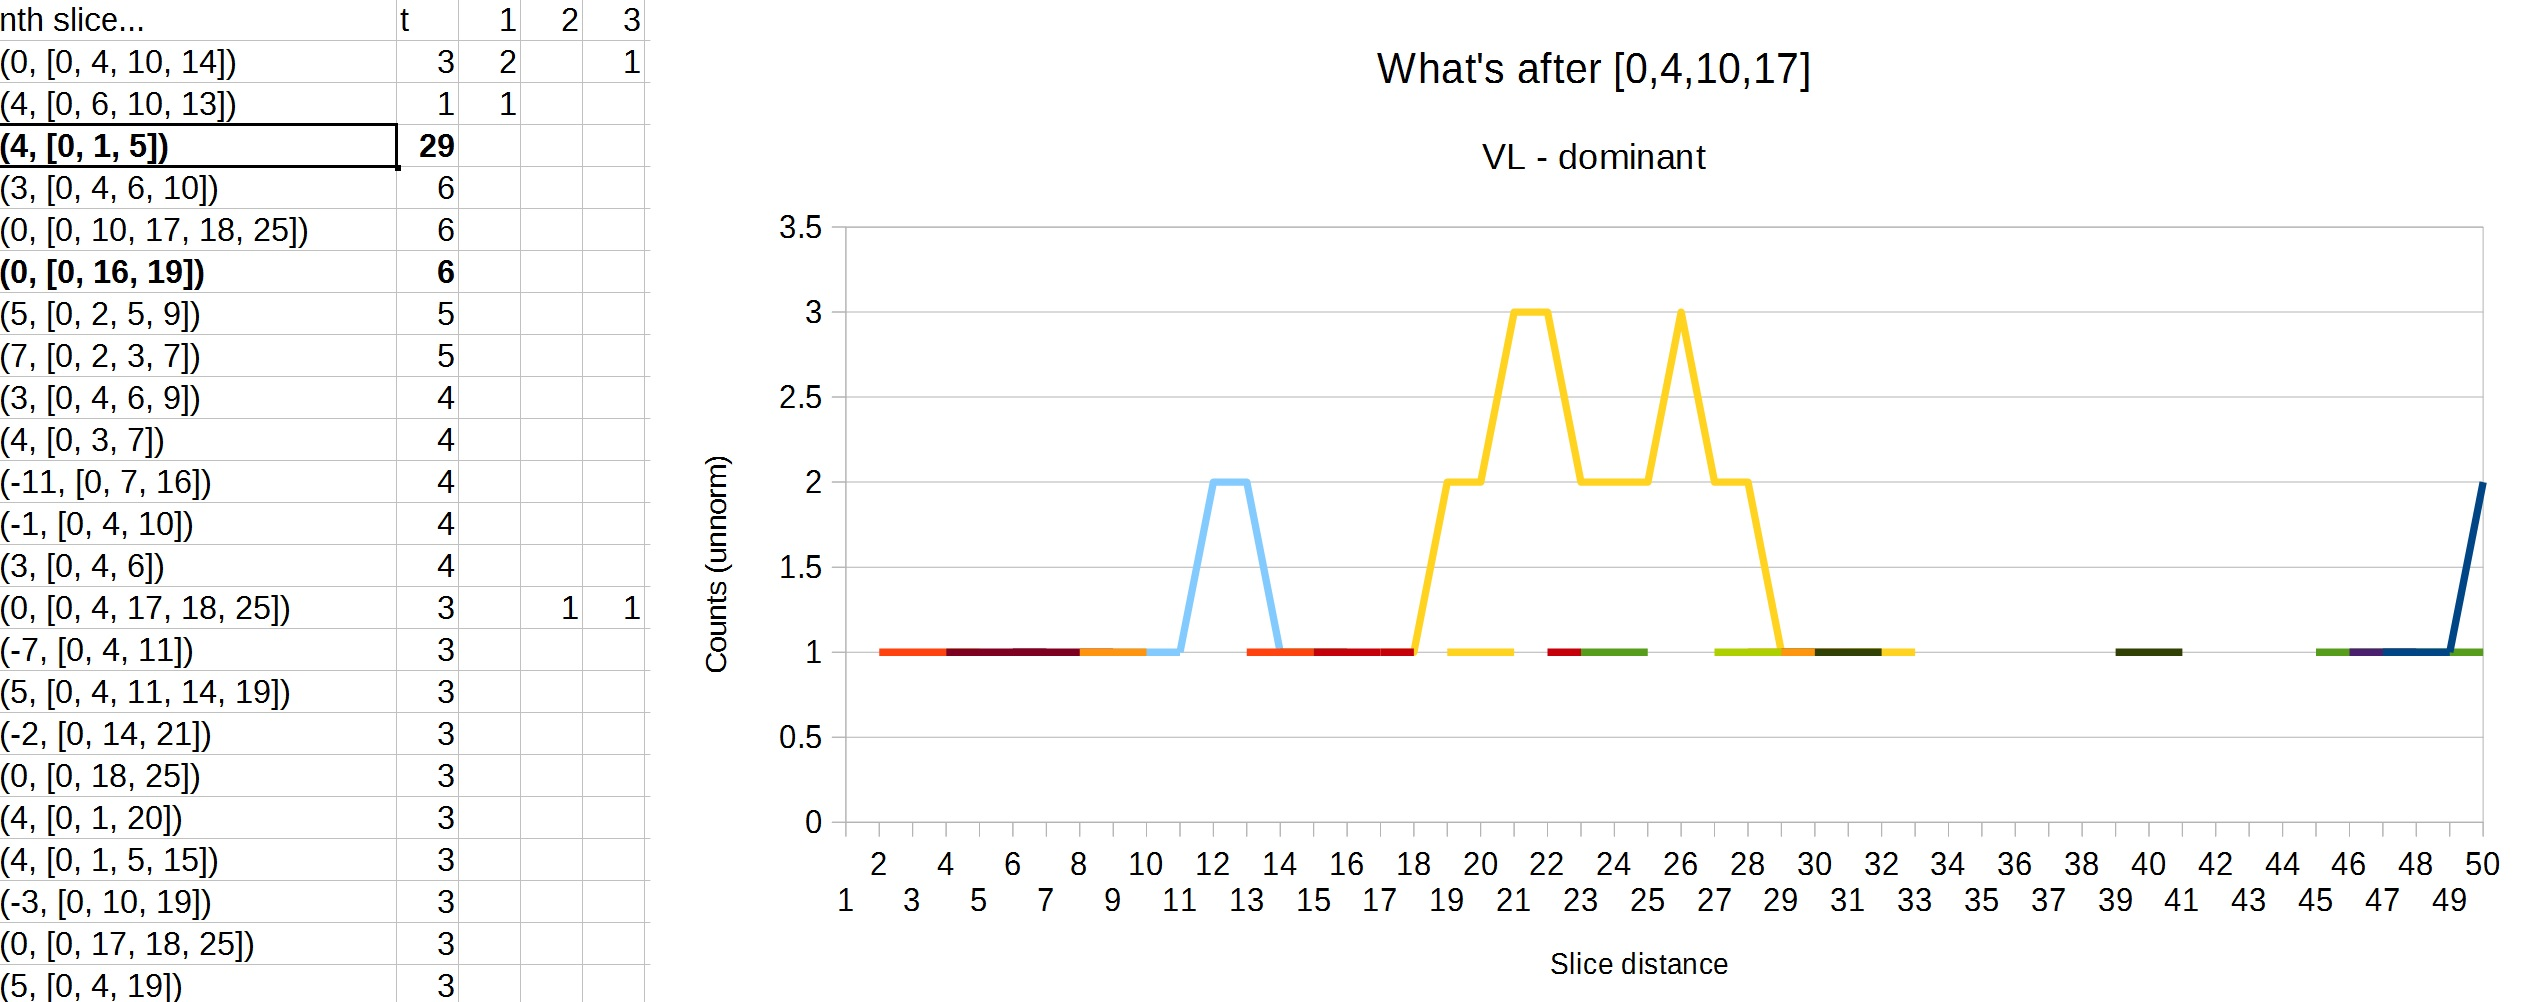
\includegraphics[width=6in]{041017_behavior.jpg}
\end{figure}

This procedure relies on a particular type of descriptive and explanatory model, and it still encodes analytical (and ontological) preconceptions regarding chord structure and harmonic progression.  To produce claims of this kind, there must exist a small number of frequently-employed chords of some ideologically-approved structure (i.e., seventh-chords with approved extensions and alterations) and a set of reduction techniques designed to render sounding sonorities of other types analytically (or at least syntactically) unimportant.  Identifying a voicing and deducing the properties of voicing types requires some minimal ontological framing, and other harmonic tasks may or may not be possible within the same frame.

\section{Selecting Objects of Harmonic Significance}
%Introduce and unpack Kockelman's semiotic diamond
The analytical pathway from abstract seventh chords to actual voicing statistics given in the preceding section relies on a selection process similar to those captured by \cite{kockelman2013} in his Figure 2.6, reproduced as Figure~\ref{kockelman} below. 

\begin{figure}[h]
	\centering
	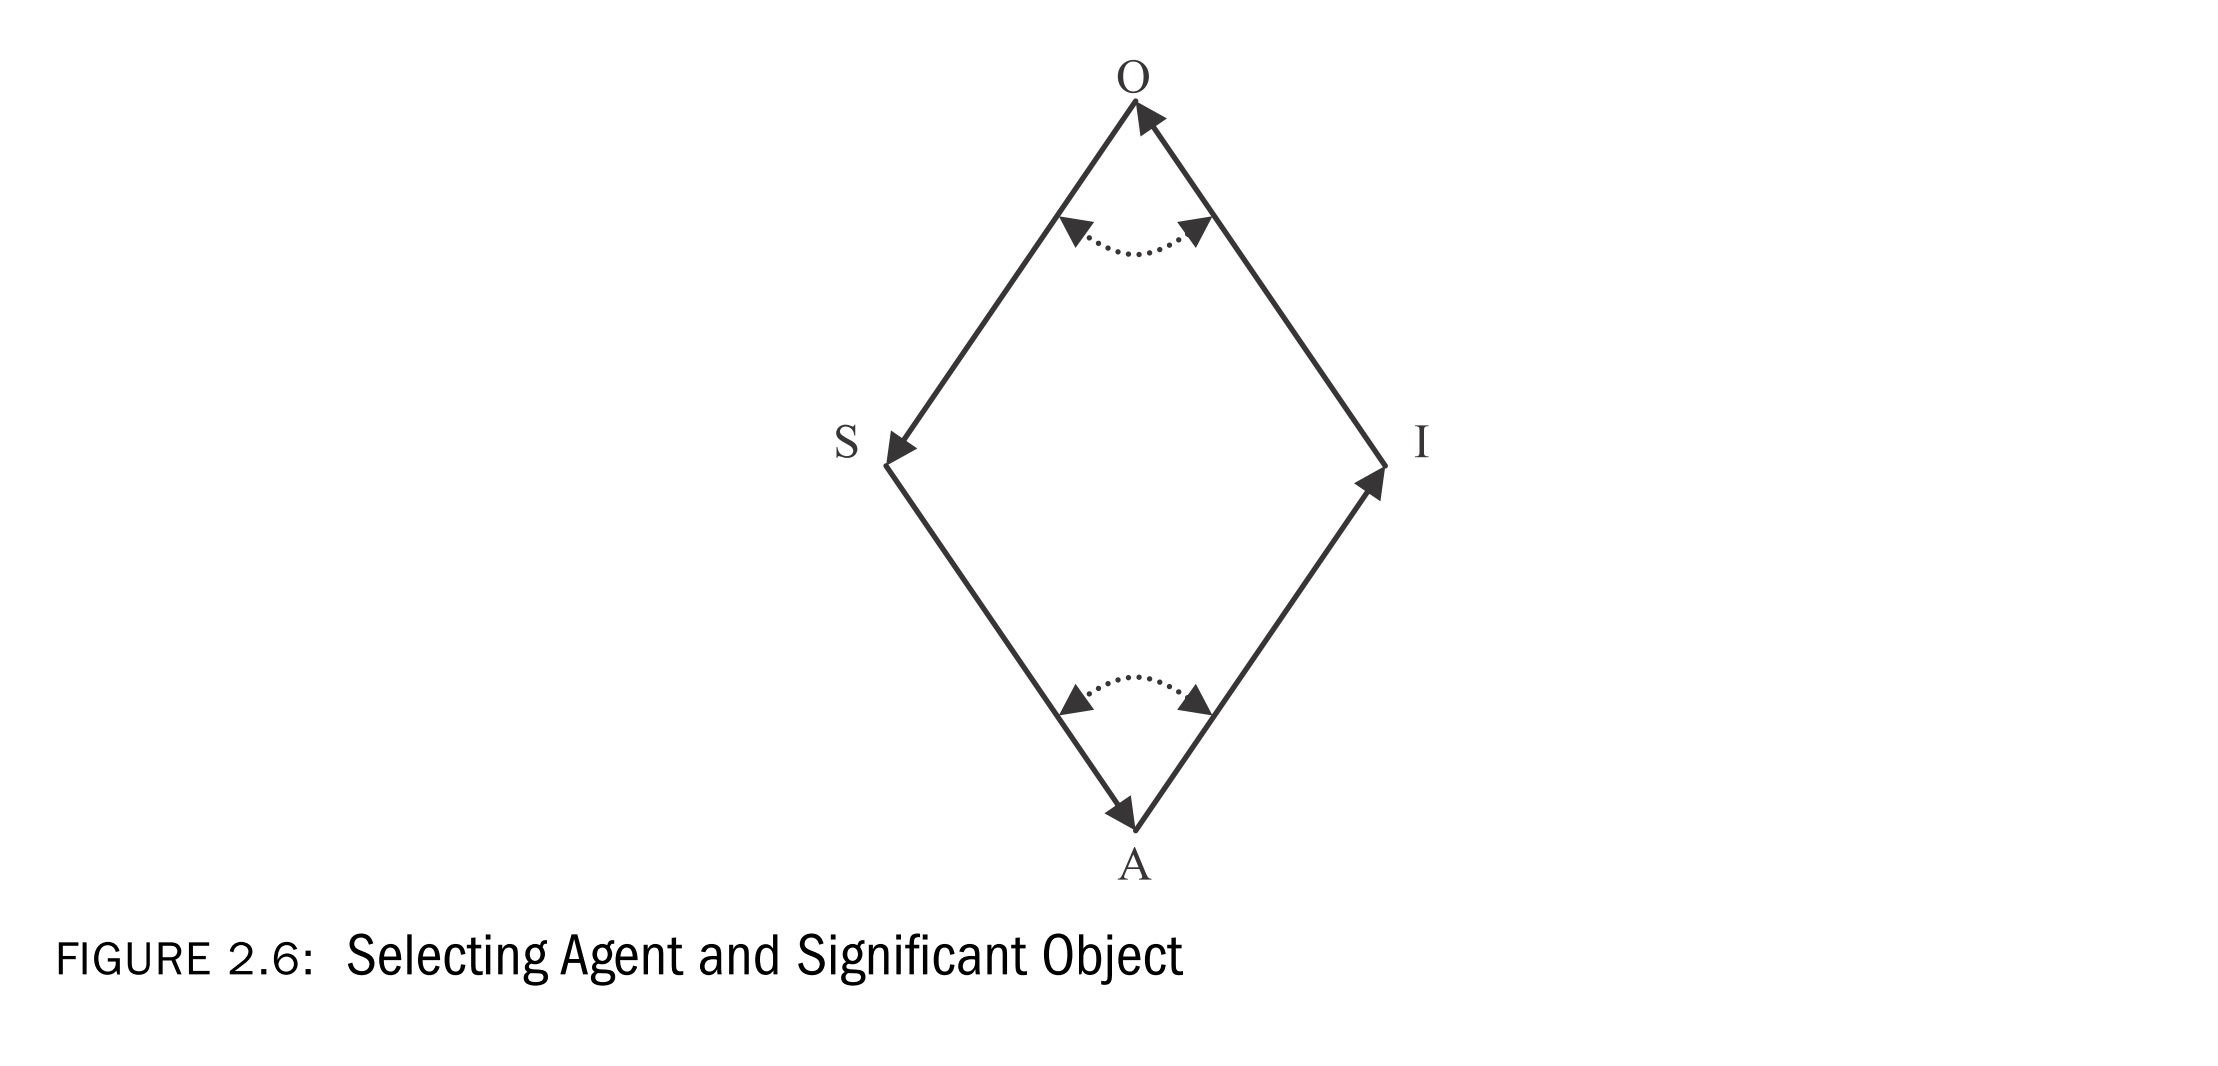
\includegraphics[width=6in]{kockelman_model.jpg}
	\caption{Figure 2.6 from \cite{kockelman2013}, a general model for the ``relation between relations" inherent in selection.  The significant object (O) and selecting agent (A) are codetermined by their relations to observable signs (S) and resulting interpretants (I).}
	\label{kockelman}
\end{figure}

This figure diagrams a flexible kind of ontological framing for semiotic processes involved in labeling, interpretation, and analysis in general.  At the top and bottom corners of this diamond, music analysis like that of the previous section places the abstract chord objects ($O$) postulated as harmonic categories (like Martin's ontologically-basic seventh chords) and the analytical agent seeking to identify, transform, and react to those objects ($A$).  The analyst does not observe the postulated objects ($O$) directly, but rather through certain traces or signs ($S$) found in the performance data, whether the engagement with those performances is acoustical (for a listening agent or pianist), visual (for a score analyst), or digital (for a corpus analyst).  The analyst observes these signed traces and produces interpretants ($I$) that make sense given the presumed existence of $O$.  These interpretants might be roman numerals that an analyst assigns to particular sonorities to represent the category of harmonic object to which they belong, or they may be expectations regarding subsequent objects which might be sounded in a performance, among other possibilities.

In a very basic analysis, the analyst might encounter a root-third-seventh voicing like $[0,4,10]$ and interpret it as a sign $S$ for an abstract (and inherently unobservable) ``dominant seventh chord" object $O$.  The analyst might then apply a roman numeral interpretant like $V^7$ to a particular location in the score and begin looking for the next syntactically-appropriate chord.  For Kockelman, the interpretant ``makes sense in the context of $S$ from the standpoint of $A$."\footnote{\cite{kockelman2013}, p.\ 17.}  The agent/analyst $A$ selects certain indices $S$ by turning signs into actions.  But Kockelman also describes the properties of the \emph{object} through a parallel and codetermined process: just as the interpretant $I$ makes sense from the standpoint of $A$ in the context of $S$, ``$I$ makes sense in the context of $S$ given the properties of $O$."  Here, $V^7$ only ``makes sense" in the context of $[0,4,10]$ if the roman numeral object has properties like identifiable root, chord structure, relationship to a key, surface segmentation, and so forth.  The resulting ``relation between relations" (the dotted lines of Figure~\ref{kockelman}) underpins semiotic processes of selection and significance, since the sense-making of $I$-given-$S$ requires and produces both a selecting agent and a significant object -- though the ontological structure from which the object $O$ arises can only be accessed, described, or interpreted by $A$ indirectly, through actions based on signs.

The flexible framework of Figure~\ref{kockelman} applies to a huge variety of selection processes, including many contexts where musical actions are taken.  In the case of actual performance, a jazz vocalist may interpret heard sonorities $S$ as indicating that a pianist is playing a kind of dominant seventh chord object $O$, and the vocalist might then choose to sing certain notes well-suited to that chord and expect and prepare for certain kinds of (say, tonic) sonority to sound after a particular time delay.  The fact that these actions make sense from the perspective of the singer (given the original heard sonority) is thoroughly entangled with the fact that the resulting actions make sense with respect to the properties of $O$ given the presence of $O$'s significant indices $S$.

Crucial to Kockelman's description of selection and significance is the claim that all agents performing (re)actions \emph{must do so under some ontological assumptions}, whether they are conscious or unconscious, enminded or embodied.  For an analyst to assign a roman numeral to a sonority, the analyst must partake of an ontology in which a variety of sonorities map to each roman numeral on the basis of their pitch class content as tokens of a type or individuals of a kind.  The analyst's interpretant (i.e., ``$V^7$," or ``look for a subsequent tonic") makes sense if and only if the kind ``dominant seventh chord with a root on scale degree five" has properties underpinning the identification of sonority/sign $S$. To use recursive language echoing Kockelman's own descriptions, the relation between the analyst-interpretant relation and the sign-analyst relation mirrors the relation between the interpretant-object relation and the object-sign relation.  Selecting a labeled kind correlated to a set of signed indices relies on and produces an ontological system.  

%Modes of ontological transformativity
Kockelman's careful attention to signed indices and acted interpretants as integral components of semiotic processes allows him to typologize their potential ontological impacts.  Consider three ``modes of ontological transformativity," to adapt part of Kockelman's typology to a music-analytical case:\footnote{The most direct analog to this discussion surrounds Table 1.2 in Chapter 1 of \cite{kockelman2013}.}
\begin{enumerate}
	\item The presence of certain notes in a voicing may change the analyst's ontological assumptions about what kinds constitute and apply to the individual sonority: ``The sign $[0,4,10]$ makes me think this sonority is a dominant seventh chord."
	\item The presence of certain notes in a very large number of similar voicings may change the analyst's ontological assumptions about what notes or intervals make up a particular kind: ``Many sonorities seem similar to $[0,4,10]$ in some important way but carry indices $[0,4,10,15]$, so perhaps a property of dominant seventh chords as a kind is that they may contain a $\# 9$ above the bass."
	\item The presence of certain unfamiliar voicings in frequent but unfamiliar patterns may change the analyst's assumptions about what voicings and harmonic objects make up a particular style or musical world: ``Many voicings do not neatly align with qualities of seventh chord, so perhaps seventh chords are not the objects (or are not the \emph{only} objects) I should react to or label."
\end{enumerate}
Transformations of type (1) here correspond most directly to undergraduate-style harmony assignments, where student analysts map observed traces to stable, received chord categories.  Transformations of type (2) constitute much of the academic music theory literature, where professional analysts logically induce pitch-based patterns of behavior from a particular corpus given a mostly-stable set of ontological kinds.  Both of these modes of ontological transformativity are well-suited to corpus analysis relaying on the ``numerical methods and explicit algorithms" Gjerdingen describes as appropriate for two-thirds of his recipe.  Gjerdingen's bias objection primarily concerns transformations of type (3), where the categories signed and represented by the statistically-tallied indices themselves change.  And the avoidance of such changes is impossible, since selecting agents produce and are imbricated in their own ontologies -- to get any selection and response procedure off the ground, the analyst must encode some set of ontological assumptions.  Where Gjerdingen says this reveals a ``presentist or historicist bias," we might say that this reveals the necessity (and inescapability) of ontological framing in analytical processes.

%aligning relations between relations
If the properties of the object ($O$) and the actions of the agent ($A$) are entangled across a semiotic process of selection and significance, the signed indices ($S$) to which the agent reacts ($I$) may be framed in a variety of ways; analysis will not consist of unearthing pre-existing harmonic objects, but rather of framing a harmonic ontology in which the properties assigned to chord objects align with the interpretants produced by the agent(s).  Different agent-interpretant relations -- different types of action or expectation taken or embodied by the analyst -- may relate more directly to certain kinds of object-sign relation than to others.  This alignment of relations between relations guides the framing of this dissertation and results in a close focus on the relays between computational category formation and temporal statistics.

\section{Harmonic objects and interpretants}
%lay out several analytical interpretants and the object-sign framings best related to them
Modes of harmonic analysis with different interpretants and objects can be framed accordingly.  Four are shown in Table~\ref{frames}.
\begin{table}%[h]
  \caption{Four framings of harmonic analysis generating (and requiring) different semiotic ontologies.}
  \centering
\begin{tabular}{>{\raggedright}p{1.6in} |>{\raggedright}p{1.8in} | >{\raggedright\arraybackslash}p{1.8in}}
\hline\hline
Interpretant & Signed Indices & Harmonic Object \\ [0.5ex]
\hline
Identifying a voicing structure & Intervals above the bass at a particular time & Pitch verticalities \\ \hline
Postulating a scale & Pitch class frequencies over time & Macroharmonic collections \\ \hline
Assigning a traditional roman numeral & Keys, pitch-class sets, reduction rules & Tertian scale degree stacks \\ \hline
%Choosing a key & Scales and articulated centricity & Tonics and modes \\
Interpreting a chord's syntactic function & Scale degree sets over time & Categories of similar scale degree sets \\[1ex]
\hline
\end{tabular}
\label{frames}
\end{table}
An analyst seeking to identify a type of voicing, following the directions of Martin and Levine, assumes (and produces) a class of pitch verticalities ($O$); the decision to place a given sonority into such a class (be they quality-based, cardinality-based, or otherwise) makes sense to the analyst given its intervals above the bass ($S$) and the existence of voicing classes ($O$) with certain intervals above the bass as properties.  This analytical process requires minimal temporal data, as the sonority's voicing structure can be gleaned from an extremely brief snapshot of a score or fragment of an audio recording, but it still assumes some temporal properties as the basis for its ontology: voicings as pitch verticalities are typically represented as simultaneities, when actual performance traces will surely exhibit slight onset time differences between each of the notes ``in" a voicing.

On another temporal scale, an analyst postulating a scale underpinning a certain passage of music assumes (and creates) limited macroharmonic collections of pitch classes that can be related to musical surface signs in particular ways; if pitch-class distributions can lead the analyst to produce a scale, then the scale object can be given such a surface distribution as a property or signed index.  In this case, as in the voicing case, the method by which the agent produces an interpretant from signed indices aligns with the properties assigned to the objects in the resulting semiotic ontology.

To assign a roman numeral or interpret a chord's syntactic function requires a more complex ontology, where the semiotic relations between the objects' properties and the agents' interpretants become less direct.  For a traditional roman numeral to ``make sense" to an analyst, she must postulate the existence of keys and pitch-class sets standing in some relation to one another.  To label the (untransposed) pitch class set $[0,4,10]$ as $V^7$ is also to assume (or create) a kind, ``$V^7$," connected to signed indices in some meaningful way.  The nature of this connection, the sense-making of ``$I$ in the presence of $S$ given the properties of $O$," is codeterminate with the with the sense-making of ``$I$ in the presence of $S$ from the perspective of $A$."  The precise way in which the analyst turns surface signs into interpretants (analytical symbols and expectations) may be thought to generate (and respond to) the way harmonic object categories relate to their signed indices (pitch and temporal properties) -- undermining any assumptions regarding the ``real" or analyst-independent nature of chord categories $O$.

On this basis, roman numeral analysis as an interpretive act fractures into several separate semiotic processes with their own distinct ontological conditions.  If the analytical interpretant produced ($V^7$) makes sense to analyst $A$ because it consists of a tertian stack of dominant seventh quality built on scale degree $\hat{5}$ of the local key, then the semiotic kind to which the individual sonority has been assigned carries properties based solely on its pitch class structure and relation to a key.  But if the same analytical interpretant is produced through some other relation to pitch and time indices, the kind $V^7$ may participate in an entirely different ontology permitting entirely different properties and modes of proof.  In particular, if $V^7$ makes sense to analyst $A$ \emph{because the observed sonority ``behaves like" other chords of kind $V^7$}, the ontological structure embedding the kind $V^7$ changes quite radically.  The relation between kind $V^7$ and its indices can no longer be captured by pitch class structure and key relation; instead, it requires additional -- and potentially conflicting -- knowledge about temporal progression or syntactic function.  As the last line of Table~\ref{frames} indicates, the interpretation of a chord's syntactic function treats more than a sonority's pitch structure as indices; such an interpretant also involves the agent's knowledge regarding what chords tend to succeed the given sonority at certain time scales.

The same human analyst may produce interpretants over-determining the properties assigned to harmonic categories at various levels of ontological transformativity.  Observing a chord's pitch-class structure or that it almost always precedes a stable tonic might lead the analyst to recognize it as part of the kind $V^7$, an ontological transformation of mode (1) above.  Or the repeated observation of those indices might lead the analyst to decide that they stand as properties of the kind $V^7$, a mode (2) transformation.  Or the analyst's concern that many chords which display some of the expected indices but not others (say, common progression behavior but unfamiliar pitch class structure) might lead to a re\"{e}valuation of the ontology framing the kind $V^7$, producing a kind category at a higher (or overlapping!) ontological level like ``dominant function," where progression behavior constitutes the signed indices producing interpretants, relegating exclusively pitch-structural indices to kinds like $V^7$.  In such an ontology, interpretive acts like ``this chord is a $V^7$" and ``this chord has dominant function" would partake of separate ontologies, rely on distinct types of evidence, and involve different analytical skills.

%transition to particular corpus-analytical harmonic analysis framings.
Some of the most-maligned limitations of computational methods -- their blessed ignorance of musical context and their blind reliance on the digital representation of the corpus -- can prove crucially useful for the generation of particular and consistent semiotic ontologies.  While human-generated interpretants like ``this sonority is a $V^7$" or ``this chord typically precedes tonic" can reference categories over-determined by their relation to indices of varying modality, algorithmic statistics and machine learning methods can be forced to produce interpretants which make sense only and precisely in the context of particular sets of indices.  With a Python implementation of an algorithm as agent $A$ in Figure~\ref{kockelman}, the direct relation between the sense-making of $I$ in the presence of $S$ from the perspective of $A$ and the sense-making of $I$ in the presence of $S$ given the properties of $O$ is strictly enforced.  The algorithm can only assign properties to object categories based on the input indices it observes -- it knows no other possible features of the object than the signs encoded in the corpus's representation.  

The remaining sections of this chapter provide examples for how such algorithmic work might ``object"-ify the YJaMP corpus.  Given interpretants designed to operate at different time scales and with different analytical aims, different computational processes are employed to ensure that the interpretant-agent-sign relations are precisely co-generated with the interpretant-object-sign relations.  The categories used to describe harmonic objects in the corpus generate different ontologies in different analytical circumstances.  Statistics regarding voicings and scales suggest future analytical projects based on YJaMP or other corpora, while temporal encodings of scale degree sets lay the groundwork for the generalized harmonic progressions of chapter 3 and the syntactic category formation of chapter 4.
 
\section{Voicings revisited}
%voicings in general, supporting and complicating Levine with more ontology
To return to the voicing statistics of Tables~\ref{[0,4,10]} and \ref{[0,4,10,17]}, we can now distinguish their different framings.  In the first case, the algorithm-as-analyst produced frequency statistics of different $[0,4,10]$ superset voicings as interpretants.  As a necessary correlate to these statistics, it assumed (or created) an ontology of voicing objects with particular properties: members of the category tallied contain an $[0,4,10]$ pitch subset, where the sounding pitches necessarily overlap in time (though they need not all begin at the same moment).  There are many subtle consequences of this ontology, like the fact that it captures voicings which may not have traditional syntactic significance (like $[0,4,10,17]$), or that a particular voicing might belong to a large number of categories.  Tables~\ref{[0,4,11]} and \ref{[0,3,10]} provide other interpretants from within the same framing: frequently-occurring corpus slices containing $[0,4,11]$ (major seventh) or $[0,3,10]$ (minor seventh) subsets.  These statistics contain further ambiguities of the same kind, but they generally support the added voice instructions given by Levine, among others.

%Check the text for whether I cite/explain upper structure voicings?
\begin{table}
\caption{Frequently-occurring corpus slices including $[0,4,11]$ voicing subsets.  These include traditional major seventh chords with various added tones, but also other traditional (``sus") and non-traditional ($[0,6,10,17]$) chords.}
  \centering
\begin{tabular}{l | l | l}
\hline\hline
Voicing & Counts & Potential interpretation \\ [0.5ex]
\hline
$[0, 4, 11]$ &	197 & \\ 		
$[0, 4, 7, 11]$ &	144	& Add \nth{5}	\\ 	
$[0, 4, 8, 11]$	& 124	& Add $\sharp$5 or $\flat$6\\ 	
$[0, 4, 6, 11]$ &	115	& Add $\sharp$4	\\ 	
$[0, 4, 5, 9, 16]$ &	89	& \nth{2} inversion, add \nth{5}, doubled \nth{7}\\ 	
$[0, 15, 19, 22, 26]$ &	80	 & Minor \nth{7}, add \nth{9}\\ 	
$[0, 15, 19, 26]$ &	62	& Minor \nth{7}, add \nth{9}\\ 	
$[0, 5, 9, 16]$ &	61	& \nth{2} inversion, add \nth{5}	\\ 	
$[0, 1, 5, 12]$ &	57	& \nth{3} inversion	\\ 	
$[0, 6, 10, 17]$ &	57	& (?)	\\ 	
$[0, 16, 20, 24, 27]$ &	52 & US $\flat$VI	\\ 	
$[0, 4, 8, 12, 15]$ &	51	& US $\flat$VI	\\ 	
$[0, 10, 14, 17, 21]$ &	49	& Sus chord	\\ 	
$[0, 10, 14, 21]$ &	48	& Sus chord	\\ 	
$[0, 8, 12, 16, 19]$ &	45	& (?)\\ 	
$[0, 2, 4, 11]$ &	44 &	Add \nth{9}	\\ 	
$[0, 10, 14, 18, 21]$ &	38 & US II	\\ 	
$[0, 1, 5, 8, 12]$ &	38 & Doubled \nth{7}\\[1ex]	 
\hline
\end{tabular}
\label{[0,4,11]}
\end{table}

\begin{table}
\caption{Frequently-occurring corpus slices including $[0,3,10]$ voicing subsets.  These include traditional minor seventh chords, with various added tones, as well as several voicings of ``sus" chords.}
  \centering
\begin{tabular}{l | l | l}
\hline\hline
Voicing & Counts & Potential interpretation \\ [0.5ex]
\hline
$[0, 3, 10]$ &	198	& \\ 
$[0, 7, 10, 17]$ &	93	& Sus\\ 
$[0, 3, 7, 10]$ &	91	& Add \nth{5}\\ 
$[0, 3, 5, 10]$ &	84	& Add \nth{4}(?)\\ 
$[0, 7, 10, 14, 17]$ &	58	& Sus\\ 
$[0, 4, 7, 14]$ &	46	& Major \nth{7}, add \nth{9}\\ 
$[0, 2, 5, 12]$ &	41	& Doubled \nth{7}\\ 
$[0, 7, 10, 12, 14, 17]$ &	41	& Sus\\ 
$[0, 7, 10, 14, 15, 17]$ &	39	& Minor \nth{11} or Sus\\ 
$[0, 3, 10, 15]$ &	38	& Doubled \nth{3}\\ 
$[0, 3, 10, 17]$ &	32	& \nth{11}\\ 
$[0, 3, 5, 7, 10]$ &	29	& Add \nth{4}(?)\\ 
$[0, 3, 7, 10, 14]$ &	29	& Add \nth{5} and \nth{9}\\ 
$[0, 16, 19, 23, 26]$ &	28	& Major \nth{9}\\ 
$[0, 3, 10, 14]$ &	28	& Add \nth{9} \\[1ex]	 
\hline
\end{tabular}
\label{[0,3,10]}
\end{table}

The categories produced by the algorithmic statistics carry no necessary syntactic properties, since the tallying process relied only on snapshots pitch alignment in time.  Even the quality of the resulting sonorities cannot be consistently determined; without knowledge of the local key and harmonic context, the root of a voicing like $[0,4,8,11]$ from Table~\ref{[0,4,11]} could be the bottom voice (0), in which case the chord contains a major third (4), sharp fifth (8), and major seventh (11), or it could be the second from bottom voice (4), in which case the chord contains a major third (8), perfect fifth (11), and flattened sixth (0).  There are good reasons to prefer the former interpretation over the latter, but the flexibility of tertian-stack quality and root identification renders both possible.  Since the voicing tally algorithm knows nothing about root or quality label, it remains agnostic regarding many potential chord properties: membership in the superset voicing category $[0,4,11]$ does not require major seventh quality, any particular root, or any particular syntactic function.

The category membership nevertheless implies some of those properties to a human analyst in a productive way, but this is to partake of a separate semiotic process diagrammed in Figure~\ref{kockelman_2dia}, taken from \cite{kockelman2013}.  The tallying algorithm $A_1$ observes voicing indices $S_1$ and produces superset statistics $I_1$ which make sense given the intervallic properties of the shared subset being tallied $O_1$.  The subsequent human analyst $A_2$ observes voicing superset statistics $S_2 = I_1$ and produces interpretants $I_2$ (like the quality label ``major seventh chord") which make sense in the context of the voicing statistics \emph{and} some embodied or enminded assumptions regarding root assignment or voice-leading reduction.  Since these properties are involved in $A_2$'s production of $I_2$, we might view them as generating signed objects $O_2$ with entirely different properties from $O_1$.  The communication between algorithmic agent and human agent can (or perhaps \emph{must}) produce different ontological framings.

\begin{figure}%[h]
	\caption{Figure 2.7 from \cite{kockelman2013}, a doubly-semiotic model for ``communication between conspecifics."  If $A_1$ and $A_2$ are a voicing tally algorithm and a human analyst, the statistical point of intersection $I_1 = S_2$ connects two processes generating different objects $O_1$, $O_2$.}
	\label{kockelman_2dia}
	\centering
	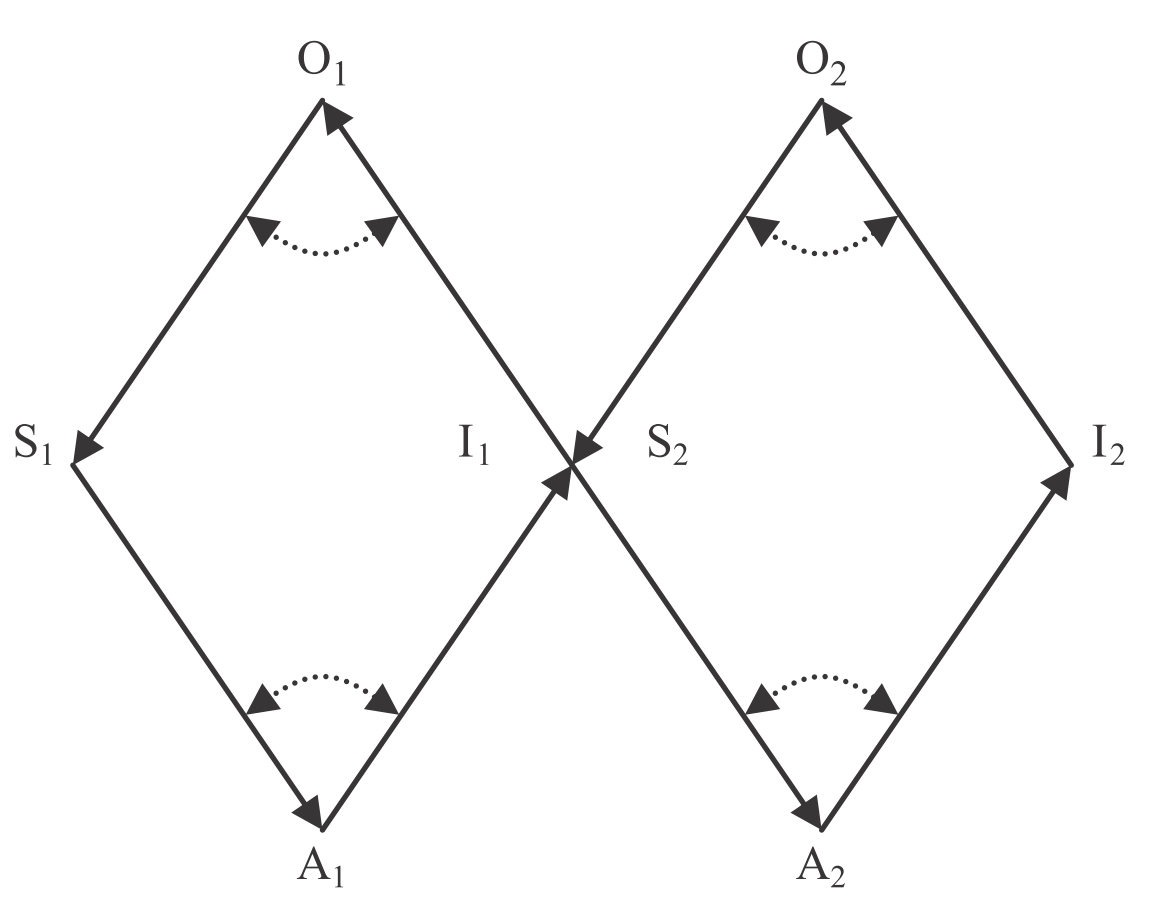
\includegraphics[width=3.5in]{kockelman_2dia.png}
\end{figure}

The potential for misinterpretation here, for ``parasitic" processes redirecting $I_1$ to some end quite different from that intended or produced by $A_1$, is clear, and it is under this condition that human-run corpus analysis must operate.\footnote{In Kockelman's terms, parasitic processes redirect or reframe semiotic processes in a variety of ways.  As formalized on \cite{kockelman2013}, p.\ 15, an object ``considered as a means to an end" (that is, as a tool for mapping $S$ to $I$) ``is a second (or an intermediary), but insofar as it implies (embodies or indexes) other ends it might be directed to serve... it is a third (or mediator).  The parasite is whatever inhabits such implications."  I will return to the implications of this claim in the concluding chapter.}  The above statistics for root-third-seventh voicing subsets imply that Levine's added tone descriptions are apt, but the price of escaping circularity in data selection is ontological instability.

Just as na\"{i}ve voicing superset tallies can be made to lend performance data driven support to three-note voicing and added tone prescriptions, the same algorithm can connect Levine's ``A" and ``B" left-hand voicings to potential chord qualities.  In Chapter 7 of his \emph{Jazz Piano Book}, Levine formalizes a harmonic progression technique designed to project $ii$-$V$-$I$ chord qualities through efficient voice leading within a single (typically left) hand voicing.  Compacting the chord changes into a single hand ``gives your right hand the freedom to play the melody or improvise," and Levine cites their occasional use by Tatum, Garner, Jamal, and Garland and attributes their codification to Bill Evans and Wynton Kelly.\footnote{\cite{levine1989}, p.\ 41.}  The left-hand voicings (LHV) present a challenge to traditional tertian-stack analysis, since they lack what Levine perceives to be the ``root" of each chord.\footnote{This is not to say that no theoretical justifications for the LHV in tertian contexts exist in the literature; Levine himself offers specific contextual justifications, while Quinn provides a general framework flexible enough to account for the LHV with generic intervals and contrapuntal rules (see \cite{quinn2017}, \S 4).}  While a bass player may pick up the roots during combo gigs, the LHV have nevertheless become a fixture of solo piano performance, and they appear frequently in the YJaMP corpus.  The two sets of efficient LHV from Levine's chapter seven are reproduced in Figures~\ref{levine_Avcg} and \ref{levine_Bvcg}.

\begin{figure}%[h]
	\caption{The ``A" left-hand voicings from Figure 7-2 of \cite{levine1989}.}
	\label{levine_Avcg}
	\centering
	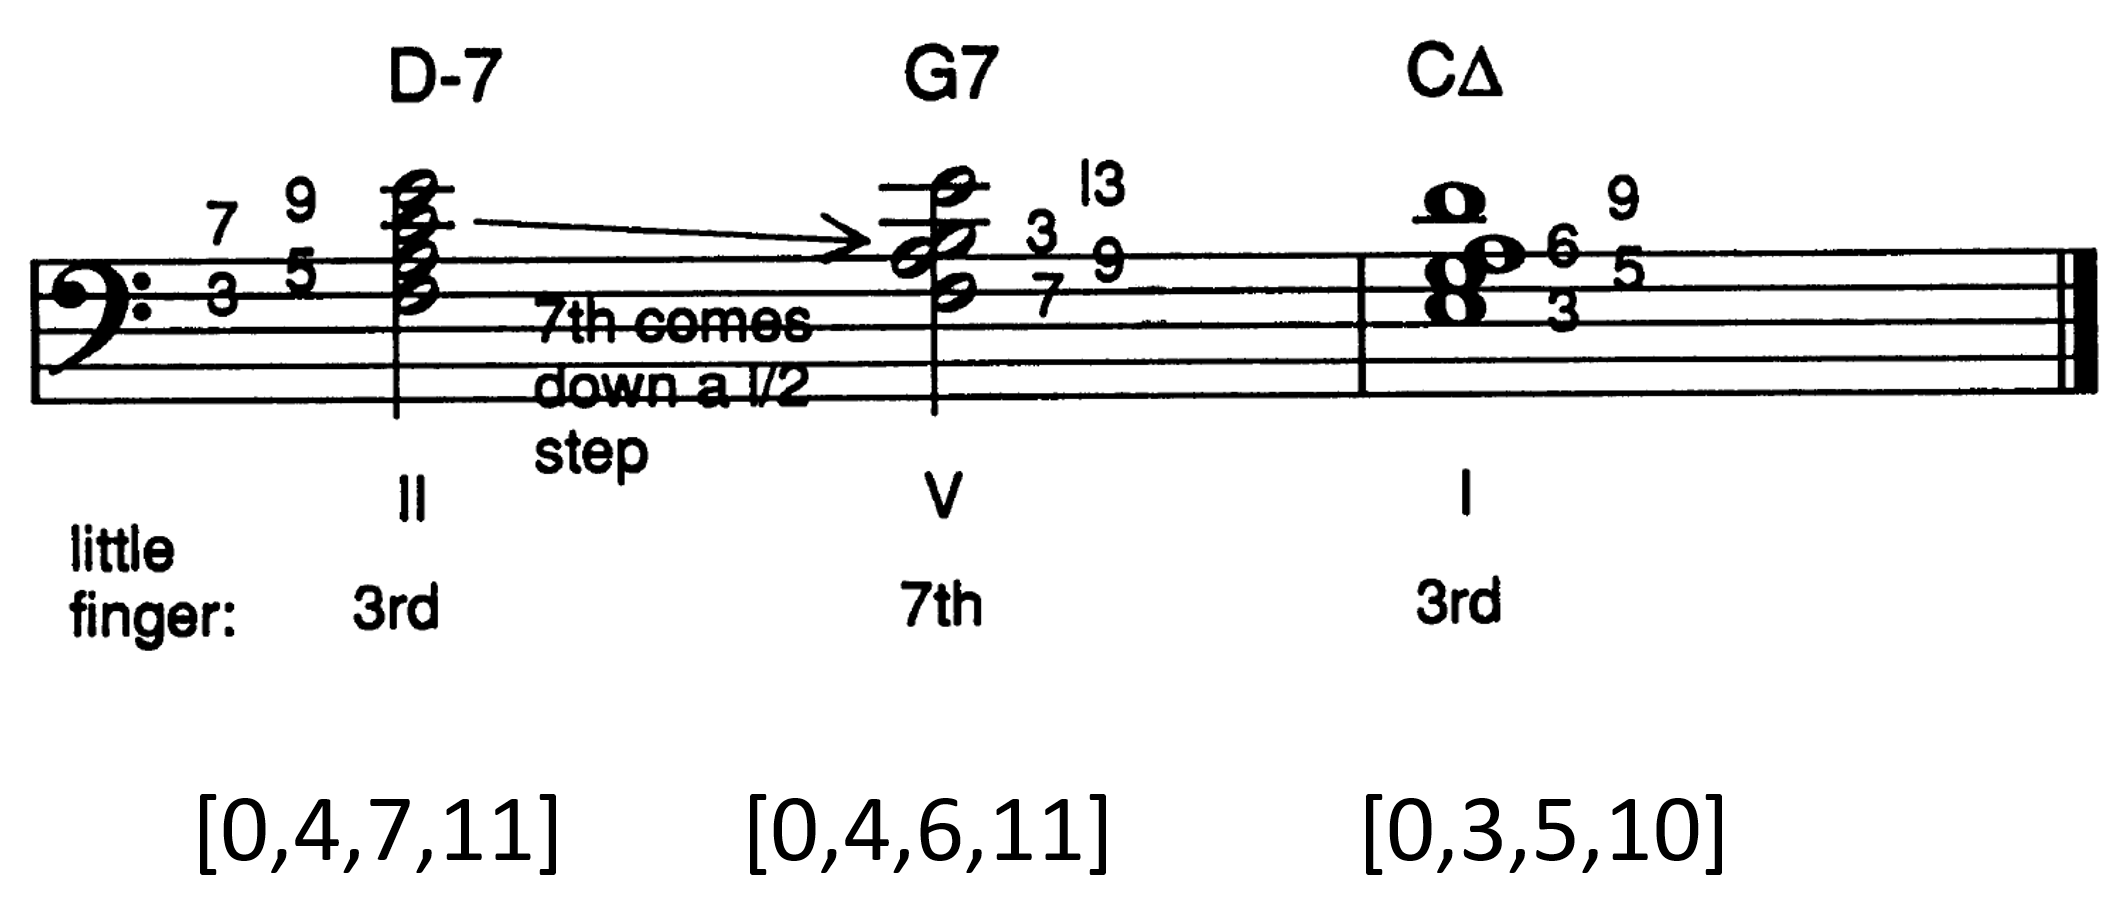
\includegraphics[width=4in]{Levine_Avoicings.png}
\end{figure}
\begin{figure}%[h]
	\caption{The ``B" left-hand voicings from Figure 7-4 of \cite{levine1989}.}
	\label{levine_Bvcg}
	\centering
	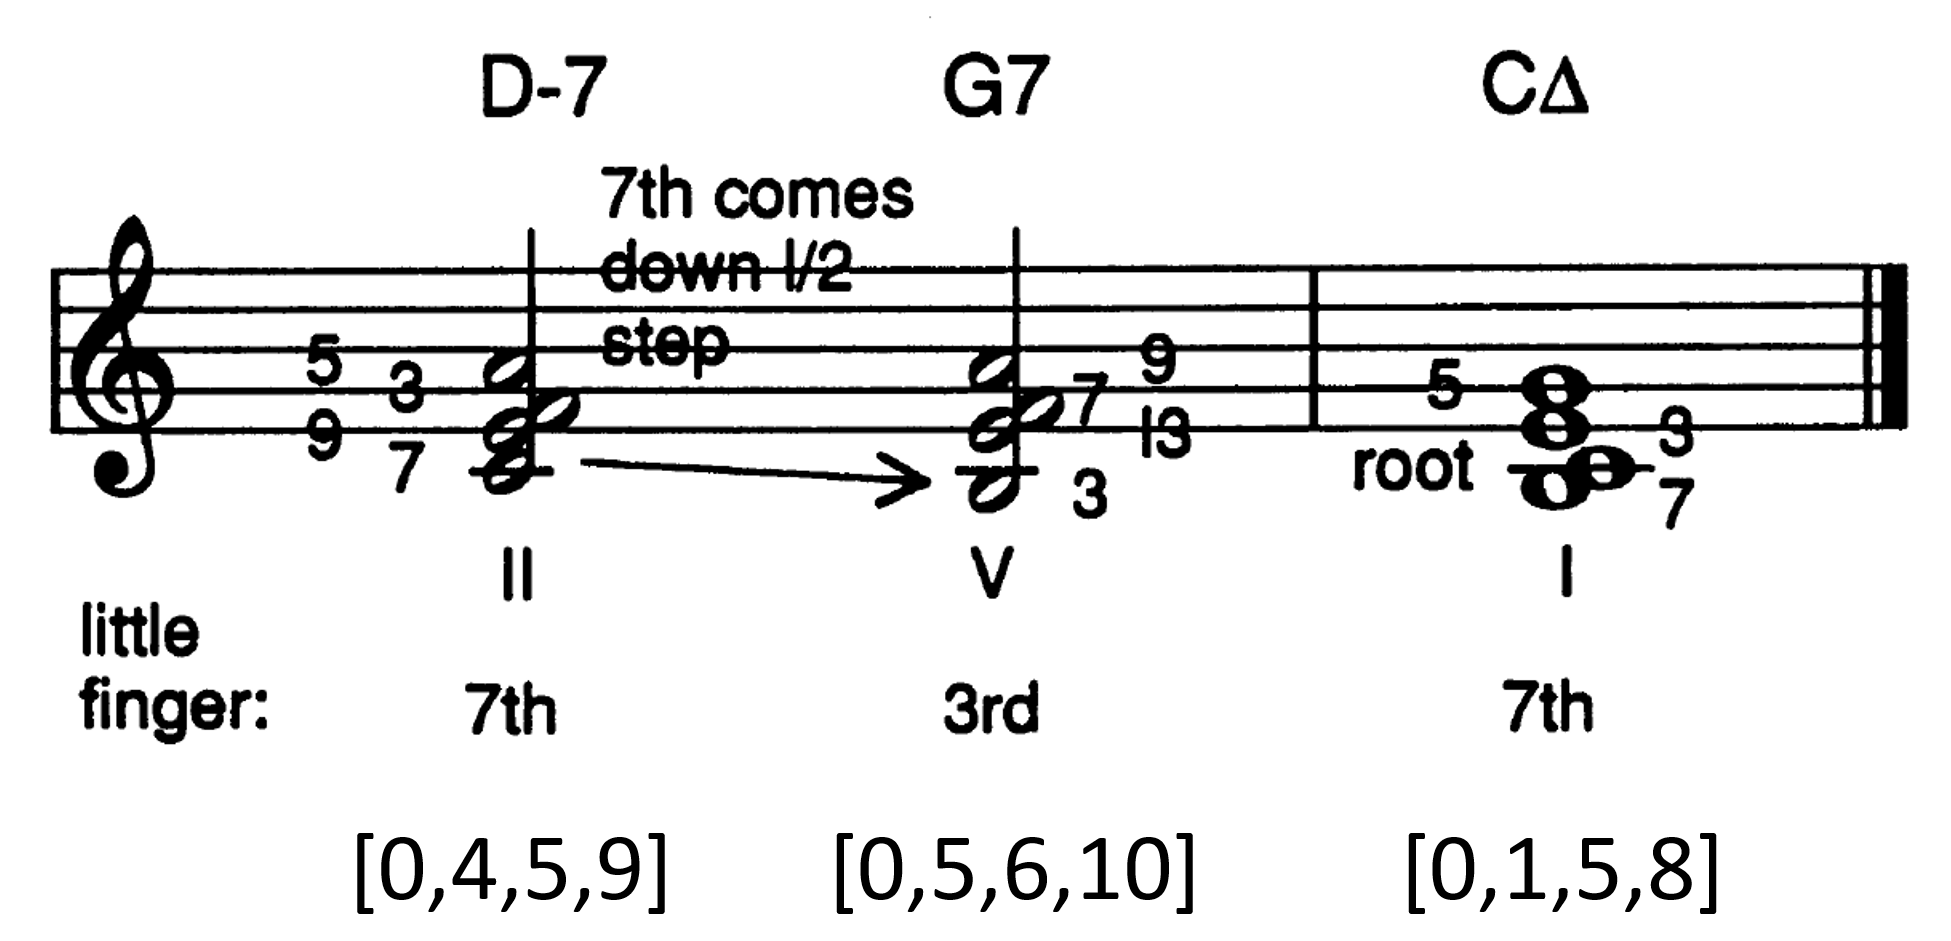
\includegraphics[width=4in]{Levine_Bvoicings.png}
\end{figure}

The intervallic structures of the A and B voicings differ from the qualities of the chords Levine intends them to index, represent, or support.  The $FM^7$ chords meant to be played in the syntactic context of ``$D-7$" can be represented with semitonal voicings $[0,4,7,11]$ and $[0,4,5,9]$, and the $G7$ voicings lack a $G$ but sound the appropriate $BF$ tritone alongside presumed chordal 9ths and 13ths.  Levine's imagined pianists run the semiotic analytical process backwards, in a way: the pianist $A$ sees chord symbols like $D-7$ or $G7$ on a lead sheet and produces voicings as interpretants.  These voicings make sense in the context of the chord symbols from the perspective of the pianist given categorical objects signed or indexed by the chord symbols: $D-7$ and $G7$ must refer to flexible collections of notes or chords for which the A and B voicings serve as adequate (or at least acceptable) responses.  Pianist-analyst communication, along these lines, might be mapped back onto Figure~\ref{kockelman_2dia}; in the left diamond, the pianist $A_1$ turns lead sheet signs into voicings ($S_1 \rightarrow I_1$), while in the right diamond, the analyst $A_2$ turns voicings back into chord symbols of some kind ($I_1 = S_2 \rightarrow I_2$).  The alignment of the framed objects $O_1$ and $O_2$ depends on the particular ways in which $A_1$ and $A_2$ make sense of their interpretants within particular (and perhaps quite different) ontologies.

To attempt to tally the appearances of Levine's left-hand voicings in YJaMP is to interpose (at least) a third diamond -- and a third agent -- into the middle of the communicative semiotic chain.  Pianist $A_1$ turns many chord symbols into many voicings; algorithm $A_2$ turns many voicings into statistics regarding common supersets; analyst $A_3$ turns those statistics into observations regarding added tones, chord quality, and categories of substitutability.  Far from collapsing the distinction between $O_1$ and $O_2$, numerical models here multiply it.  We might be inclined to tack on yet another diamond before the others, where a tune writer turns imagined, composed, or improvised sonorities into lead sheet symbols-- in which case the entire communicative enterprise might suggest a kind of philosophical fictionalism, where each agent's actions are embedded in an ontology appealing to certain kinds of harmonic objects as a convenient way to facilitate the production and communication of their own interpretants.  Embracing a music theoretical fictionalism similar to Hartry Field's nominative philosophy of mathematics would amount to claiming that roman numeral models (or chord categorical claims, more generally) provide a reliable and convenient communicative framework consisting of literal falsehoods.\footnote{I note in passing that since music theory seems to rely more heavily on first-order logic than second-order, it may be a more appropriate domain for Field's construction than mathematics, the second-order logical constraints of which have generally limited Field's acceptance by the field.  See \cite{field1980}.}  To adopt complete skepticism regarding chord categories as referring to anything existing independently in the real world would amount to a very high mode of ontological transformativity, in Kockelman's terms.\footnote{While acceptance of this position is not strictly required by my project here, I align myself in this direction, and I think it can be read out of work like \S 1 of \cite{quinn2017}.}  All this to say: using corpus statistics to assess the appropriateness of the left-hand voicings as descriptors of piano performance is like standing on a stool balanced on a chair placed on a crooked floor.\footnote{Passionate defense or criticism of musical corpus analysis seems to depend on whether one thinks the analyst in this precarious position is trying to reach the ceiling or the floor.}  So it is deceptive and surprising how straight-forward the results appear.

\begin{table}%[h]
  \caption{Supersets of of Levine's $ii$ ``A" left-hand voicing (LHV) $[0,4,7,11]$.}
  \centering
\begin{tabular}{l| l | l}
\hline\hline
Voicing & Counts & Potential interpretation \\ [0.5ex]
\hline
$[0,4,7,11]$ & 199 & Major seventh or $ii$ LHV\\
$[0,15,19,22,26]$ & 117 & LHV + added root = minor ninth \\
$[0,10,14,17,21]$ & 58 & Major ninth in inversion, or sus? \\
$[0,1,5,8,12]$ & 51 & Major seventh with doubled 7 \\
$[0,2,4,7,11]$ & 47 & Major seventh add 2 \\
$[0,3,7,10,14]$ & 36 & LHV + added root = minor ninth \\[1ex]
\hline
\end{tabular}
\label{a_ii_lhv}
\end{table}

In Figure~\ref{a_ii_lhv}, I turn the superset voicing statistics produced algorithmically for all the appearances of $[0,4,7,11]$ corpus-wide into interpretations invoking chord quality and added tones.  The most frequent voicing containing $[0,4,7,11]$ as a subset is the four-note voicing itself.  These sonorities likely occur in contexts where we might interpret them as root-position major seventh chords, so their frequent appearance neither supports nor undermines the claim that $[0,4,7,11]$ can appear in place of something like a $ii$ minor seventh chord.  But the second most common superset voicing, sounding 117 times in the corpus, resembles precisely the kind of minor ninth chord Levine suggests will result from the addition of a chord root.  The intervallic $[0,4,7,11]$ structure appears in the upper voices ($[15,19,22,26]$), and the bass of the voicing sounds a minor tenth below; if the former is a major seventh voicing, like $(F,A,C,E)$ in Figure~\ref{levine_Avcg}, then the added root produces a minor seventh chord with an added ninth, like $(D,F,A,C,E)$.  The most frequent way to add any additional voices to $[0,4,7,11]$ produces precisely the quality Levine predicts, as does the sixth most frequent ($[0,3,7,10,14]$, which reduces the minor tenth from the previous voicing to a minor third).  $[0,1,5,8,12]$ and $[0,2,4,7,11]$ could appear in the context of a major seventh or the minor seventh LHV, where the extra voice functions as a doubled seventh and added second (in the $M7$ case) or doubled ninth and added eleventh (in the rootless $m7$ case), respectively.

The quality of the third most common voicing superset of $[0,4,7,11]$ is formally ambiguous but pragmatically identifiable.  $[0,10,14,17,21]$ contains an intervallic $[0,4,7,11]$ as its upper voices and adds a bass note a minor seventh below -- if the $[0,4,7,11]$ is the $(F,A,C,E)$ of Figure~\ref{levine_Avcg}, then this added bass produces $(G,F,A,C,E)$.  An elementary harmony student might readily identify this sonority as an $F$ ninth chord in fourth inversion, while an experienced jazz analyst might point to the wide spacing between the bass and the upper voices as evidence that this label is unproductive.  The added voice bears no particular resemblance to the $ii^7$ chord suggested by Levine's LHV, but it does appear in precisely this form in his Figure 4-3, reproduced here as Figure~\ref{Gsus}.  Here, Levine annotates the figure to identify the $D-7$ LHV in the upper $[0,4,7,11]$ subset, but he describes the full voicing as an archetypal ``Gsus" chord.  As Levine explains the labeling and use of this chord, he presents the results of of a multiply-framed ontology: ``$F/G$ describes exactly what's happening... an $F$ triad in the right hand over the note $G$ in the left hand.  $D-7/G$ describes the \emph{function} of the sus chord, because a sus chord is like a $II-V$ progression contained in one chord."\footnote{\cite{levine1989}, p.\ 23.}  He attributes the popularization of sus chords to Coltrane and Hancock, and he notes that it may be used with the dominant chord produced by 4-3 resolution or without one.

\begin{figure}
	\centering
	\caption{Figure 4-3 from \cite{levine1989}, a ``Gsus chord."  The upper four voices appear in other contexts as a major seventh chord or the A LHV for a minor seventh chord.}
	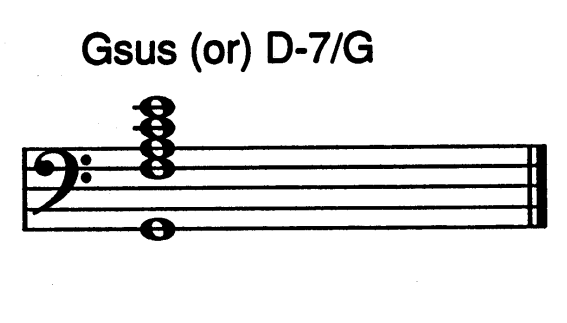
\includegraphics[width=2in]{levine_43.png}
	\label{Gsus}
\end{figure}

Levine's labels refer to (and within) two separate semiotic structures: $F/G$ is an interpretant produced by an agent (something analogous to a ``voicing algorithm" $A_1$ in Levine's brain) in response to voicing and pitch content, while a different agent (a ``function algorithm" $A_2$) uses nearly identical nomenclature ($D-7/G$) to index some property of the chord's function.\footnote{I mean this analogy to ground the semiotic processes involved in producing labels -- not as some cognitive description of Levine or any other analyst.  As Chapter 5 explains, the utter simplicity of algorithmic agents lends itself unusually well to explicit semiotic framings.}  Levine explains this function in strictly pitch-based terms -- ``your right hand plays a common $D-7$ left-hand voicing... over a $G$ root," and ``the $II-V$ progression in the key of $C$ is $D-7$, $G7$" -- but the functional interpretant is \emph{not} produced simply by analyzing intervallic voicing and pitch structure.\footnote{\cite{levine1989}, p.\ 23.}  Rather, Levine's presentation relies on a functional ontology in which $ii$ minor seventh chords have a property of leading to $V$ dominant sevenths in tonally syntactic progressions.   Despite the student analyst's observation that this sonority consists exclusively of pitch classes belonging to $F^9$, the voicing and progression behavior of $[0,10,14,17,21]$ leads Levine to produce $D-7/G$ as a functional interpretant.  

In a way, this sus-usage of $[0,4,7,11]$ remains true to the ethos of Levine's left-hand voicings.  Table~\ref{a_ii_lhv} assessed how frequently the LHV appeared as the upper voices of a minor seventh chord (typically preceding a dominant $V$, for Levine), but my interpretation of one of its statistics implied that the voicing also frequently appears as the upper voices of a sus chord (typically preceding or replacing $V$, for Levine).  In both cases, Levine carefully assigns a root to the chord, and in both cases the root is determined not by pitch content but by the typical behavior of the chord in tonal progressions.  This appeal to participation in certain kinds of syntactic progressions as a basis for the assignment of harmonic kinds will provide the basis for Chapters 3 and 4.

Figure~\ref{a_V_lhv} provides a simpler statistical portrait of the supersets for $[0,4,6,11]$, the left-hand A voicing Levine suggests for $V$.  Each of the ten most frequent appearances of a $[0,4,6,11]$ superset either (1) doubles a voice at the octave, (2) adds a chord extension appropriate to a dominant seventh with $[0,4,6,11]$ as its upper voices, or (3) adds the root required to turn $[0,4,6,11]$ into a fully-voiced dominant seventh (9,13) chord.  The superset data indicates that $[0,4,6,11]$ tends to appear in fewer contexts than $[0,4,7,11]$, both in terms of overall frequency and interpreted quality.  The voicing superset statistics for the B voicings, given here as Figure~\ref{b_ii_lhv} and \ref{b_V_lhv}, fit a similar narrative.  In each of these cases, the performance data indicates that Levine's left-hand voicings often appear as the upper voices of chords with the qualities he predicts.

\begin{table}%[h]
  \caption{Supersets of of Levine's $V$ ``A" left-hand voicing (LHV) $[0,4,6,11]$.}
  \centering
\begin{tabular}{l| l | l}
\hline\hline
Voicing & Counts & Potential interpretation \\ [0.5ex]
\hline
$[0,4,6,11]$ & 160 & LHV \\
$[0,4,6,11,18]$ & 31 & Voice 3 doubled \\
$[0,4,6,11,23]$ & 28 & Voice 4 doubled \\
$[0,2,4,6,11]$ & 23 & LHV + added root = dominant seventh (9,13) \\
$[0,4,6,11,16]$ & 22 & Voice 2 doubled \\
$[0,4,6,11,21]$ & 18 & LHV of $V$: added fifth \\
$[0,10,14,16,21]$ & 16 & LHV + added root = dominant seventh (9,13) \\
$[0,4,6,11,26]$ & 14 & LHV + added root = dominant seventh (9,13) \\
$[0,4,6,11,20]$ & 14 & LHV of $V$: added \# 11 \\
$[0,1,5,7,12]$ & 13 & Voice 1 doubled \\[1ex]
\hline
\end{tabular}
\label{a_V_lhv}
\end{table}

\begin{table}%[h]
  \caption{Supersets of of Levine's $ii$ ``B" left-hand voicing (LHV) $[0,4,5,9]$.}
  \centering
\begin{tabular}{l| l | l}
\hline\hline
Voicing & Counts & Potential interpretation \\ [0.5ex]
\hline
$[0,4,5,9]$ & 476 & Major seventh or $ii$ LHV \\
$[0,4,5,9,16]$ & 124 & Voice 2 doubled \\
$[0,4,5,9,19]$ & 107 & $ii$ LHV: added 11 or M7 add 9 \\
$[0,4,5,9,21]$ & 87 & Voice 4 doubled \\
$[0,4,5,9,17]$ & 69 & Voice 3 doubled \\
$[0,4,5,9,28]$ & 67 & Voice 2 doubled \\
$[0,7,11,12,16]$ & 65 & Voice 3 doubled \\
$[0,10,14,15,19]$ & 65 & $ii$ LHV: added root \\[1ex]
\hline
\end{tabular}
\label{b_ii_lhv}
\end{table}

\begin{table}%[h]
  \caption{Supersets of of Levine's $V$ ``B" left-hand voicing (LHV) $[0,5,6,10]$.}
  \centering
\begin{tabular}{l| l | l}
\hline\hline
Voicing & Counts & Potential interpretation \\ [0.5ex]
\hline
$[0,5,6,10]$ & 62 & $V$ LHV \\
$[0,5,6,10,20]$ & 17 & LHV + added root = dominant seventh \\
$[0,6,11,12,16,20,23]$ & 15 & Voice 3 doubled; if $V$ LHV: added \# 11, 13 \\
$[0,5,6,10,18]$ & 10 & Voice 3 doubled \\
$[0,5,6,10,17]$ & 10 & Voice 2 doubled \\
$[0,5,6,10,29]$ & 10 & Voice 2 doubled \\
$[0,5,6,10,27]$ & 8 & $V$ LHV: added fifth \\[1ex]
\hline
\end{tabular}
\label{b_V_lhv}
\end{table}

To assess the functional behavior of these chords -- whether they \emph{behave like} a $ii$ or $V$, instead of merely resembling one -- requires (more) engagement with keys and temporality.  A maximally transparent form of functional data mining would restrict itself to evidence like that given in Figure~\ref{[0,4,10,17]}, which implied local dominant-tonic relations directly from temporal voicing data and without the need to impose judgments regarding key.  But the claims of  Figure~\ref{[0,4,10,17]} are based on extremely slim data -- a handful of observations for each transition.  The pianists recorded in YJaMP use such a wide variety of voicings that tracking the progression behavior of each one individually would require a far larger corpus.\footnote{If the number of distinct voicings employed scales roughly linearly with the number of pianist-hours recorded, no corpus of any size could produce the relevant statistics.  I assume, however, that the number of distinct voicings will level off much faster than the number of recordable performances, rendering the problem accessible at large scale.}  As Levine already implies by describing ``voicings" in terms of their progression behavior relative to local key centers, transposing the wide variety of possible voicings relative to their local keys greatly reduces the size of the computational alphabet -- and generates a new ontological framing amenable to syntax.

\section{Scale degrees and key finding}

Since many corpus analysts view their computational tasks as attempts to replicate the cognitive properties of a human listener or analyst, the algorithmic assignment of keys to passages of music sits at the heart of a wide variety of otherwise disparate harmonic analysis projects.  Starting at least as early as the (human) experimental work of Krumhansl, Schmuckler, and Kessler of the 1980s, keyfinding studies typically assume that key determinations arise at least partly in response to pitch-class distributional patterns.\footnote{See \cite{krumhansl1982} and \cite{krumhansl1990}.}  Whether generated by probe-tone studies of perceived stability or key-appropriateness for particular chords and pitch classes (Krumhansl 1990), melodic pitch class statistics from the Essen folk music corpus (Aarden 2003), or polyphonic pitch class frequencies from 18th and 19th-century art music (Aarden 2003, Bellmann 2005, Temperley 2007), key profiles generally assume the form of a twelve-dimensional probability distribution indicating the likelihood or prevalence of each pitch class given a particular key.\footnote{See \cite{krumhansl1990}; \cite{aarden2003}; \cite{bellmann2005}; \cite{temperley2007}, Ch. 6.  Automated key-finding based on statistics other than pitch class distributions can also yield excellent results, as in \cite{quinn2010}, but this study constitutes a significant outlier in the literature.} The specific parameters vary from profile to profile, but the general results for western tonal repertoires tend to resemble Figure~\ref{krumhansl} (reprinted from \cite{krumhansl1990}), whether arising from perception studies or corpus statistics.

\begin{figure}%[h]
	\centering
	\caption{Figure 3.3 from \cite{krumhansl1990}.  The relative frequencies for each pitch class relative to the local tonic (given as $C$, on the horizontal axis) for several small corpora (circles, triangles, and squares) and human perception studies (diamonds).}
	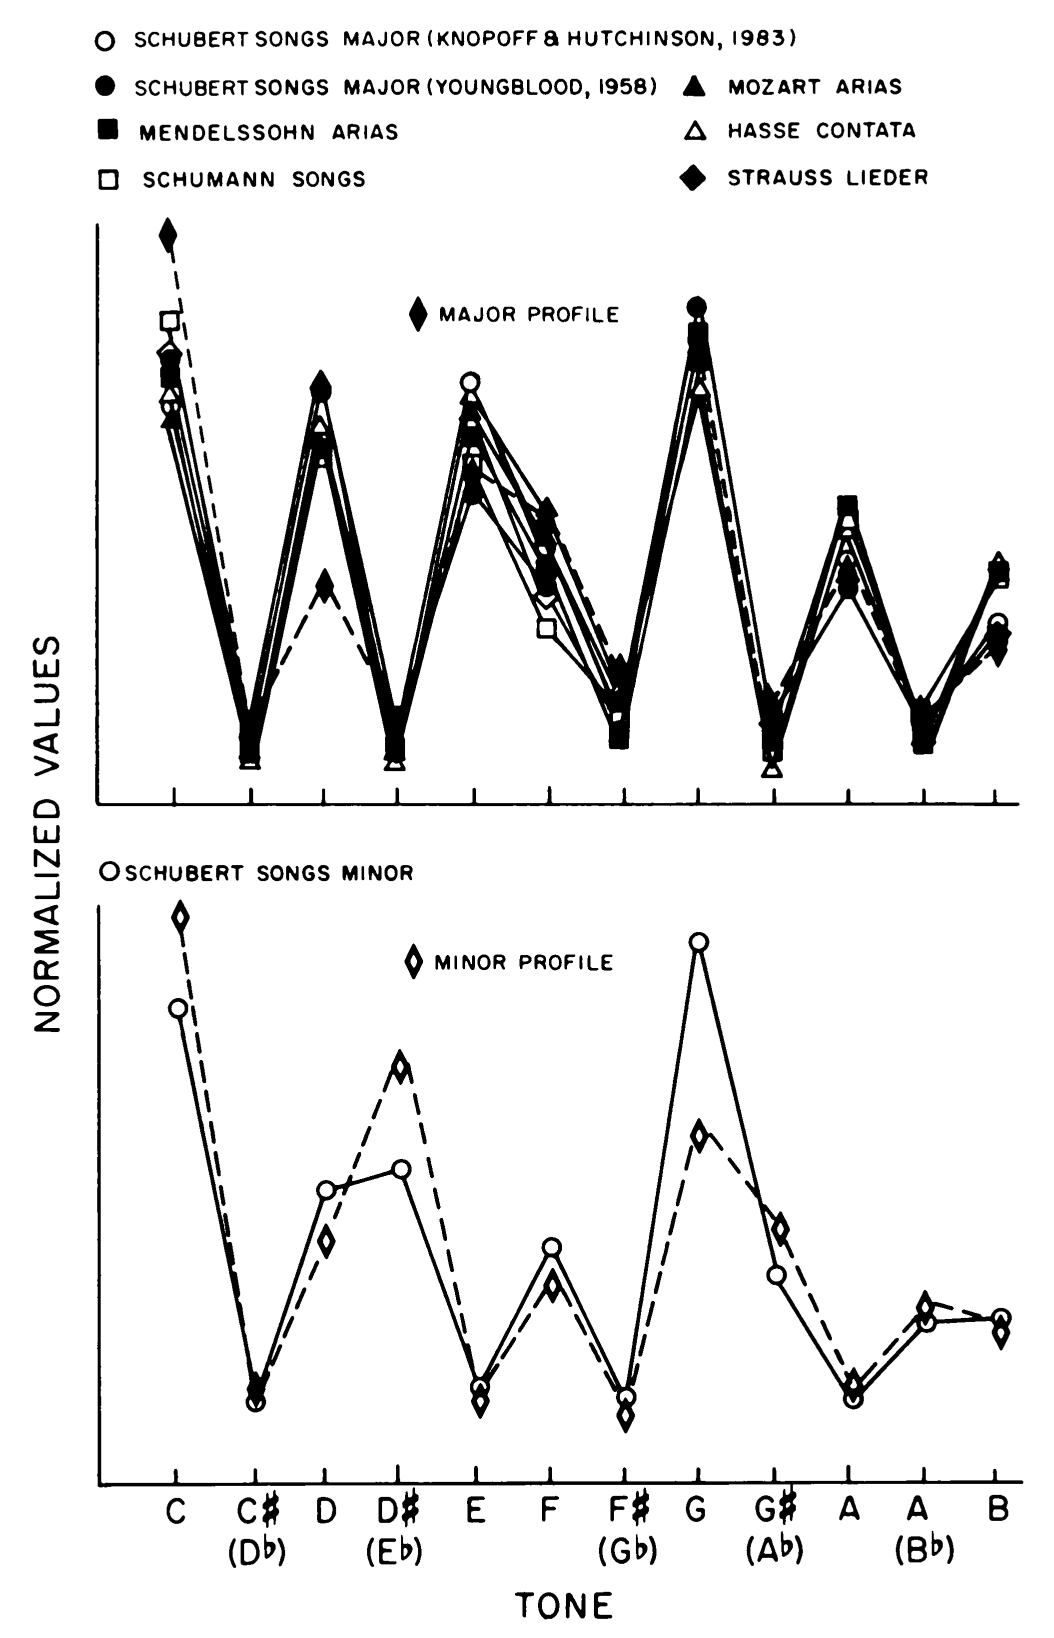
\includegraphics[width=4in]{krumhansl.png}
	\label{krumhansl}
\end{figure}

Figure~\ref{krumhansl} presents similarly-shaped profiles generated in distinct ways.  The diamond-dotted ``major" and ``minor" profiles plot a stability or goodness-of-fit rating listeners assigned each pitch class when played in the context of the relevant key.  A higher vertical axis value for these curves indicates that the experimental subjects considered the pitch class very stable or appropriate to the key, while lower values indicate the opposite.  The curves delineated by circular, triangular, or square dots plot a normalized measure of frequency of appearance for each of these pitch classes in key-analyzed corpora from different composers.  The absolute scale is unimportant -- the major contribution of Figure~\ref{krumhansl} is to indicate the relative importance of each scale degree to a local key and to show a close fit between profiles generated from perception studies and those generated from pitch class statistics.\footnote{For further experimental details, see \cite{krumhansl1982}; for wider context, see \cite{krumhansl1990}.}

Armed with these (or similar subsequent) major and minor key profiles, key-finders typically tally the pitch class distributions for a given musical passage and use some basic quantitative methods to select which assumed tonic's profile would produce the best fit.  Any key-finding algorithm written along these lines needs three essential inputs:
\begin{enumerate}
	\item A selected passage for which the key is desired but not known
	\item A set of theoretical key profiles
	\item A goodness-of-fit measure by which the statistics from (1) can be compared to (2)
\end{enumerate}
%first: the perpexity-based segmentation process
These inputs correlate to a segmentation problem, a parameterization problem, and an optimization problem, respectively.  While some studies approach segmentation (1) with broad heuristics, like using the pitches of an entire piece\footnote{\cite{krumhansl1990} or the first and last 8 measures of each piece\footnote{\cite{albrecht2013}}, others chop each piece into many parts and assign a probable key to each.\footnote{See \cite{temperley2007}; \cite{white2013}.}  As Temperley notes, segmenting a piece into many consecutive ``windows" allows a key-finding model the flexibility to identify modulations.\footnote{\cite{temperley1999}, pp.\ 78-81.}  But while Temperley makes a convincing case for the necessity of windowed segmentation in key finding, he provides no real heuristic for the determination of window size.\footnote{See \cite{temperley1999}, p.\ 81, for example, where ``Segments of about 1 measure -- typically between 1 and 2 s long -- proved to be about optimal..."  This heuristic carries over to \cite{temperley2007}.}  Most windowed key-finding algorithms choose a set number of measures, beats, or note onsets as an appropriate window, despite Temperley's caveat that ``[t]his also means that the tempi chosen for pieces may affect the program's analysis."\footnote{\cite{temperley1999}, and see also the eight quarter-note window employed in \cite{wq2017}.  Sliding these fixed windows through the corpus with an incrementing interval of a quarter note allows White and Quinn to determine modulations over durations shorter than eight quarters.}

Setting a window size by measures or beats runs the risk of attempting key assignments for segments of radically different cardinality.  Fortunately, a performance corpus like YJaMP affords the examination of timing data taken directly from note onsets, bypassing notational questions regarding measure lines, beats, or notated tempi.    Figure~\ref{cardinalities} displays the output of a simple counting algorithm;\footnote{This windowing code and other key-finding methods discussed here are available at \href{github.com/andrewdjones/YJaMP_Analysis}{github.com/andrewdjones/YJaMP\_Analysis}.} for temporal window sizes of 400ms, 800ms, 1.6s, and 3.2s, the algorithm tallies the number of windows with each pitch-class cardinality corpus wide.  On average, 400ms windows tend to capture pitch-class sets of cardinality 3-5, the smallest cardinalities at which we might expect to find traditional chord objects carrying harmonic information, while windows of longer duration gradually increase in average cardinality.  Windows of 1.6 seconds tend to contain about 7 pitch classes -- the start of what we might call the scalar regime -- and 3.2 second windows begin to approach the 12-tone aggregate.

The smooth logic of these curves hides reasons for the key-finder to worry.  If the corpus is segmented into 400ms segments, some of them will contain only two pitch classes -- likely too few for any meaningful key assignment -- while others contain seven or eight.  Algorithms segmenting windows based on a particular number of note onsets might seem to solve the problem, but they prove highly sensitive to repetitions and decorative figurations.\footnote{For an example of repetition-sensitivity for small windows, see Chapter 6 of \cite{temperley2007}.  While Temperley advocates ignoring repetitions to mitigate the problem, I retain this information and adjust the window sizes accordingly.}

To account for both disparities, I employ a key-finding algorithm with a variable window size set through distributional means.  Collections of pitches well-suited to key-finding will contain an instance or two of several pitch classes, consisting neither of one pitch class (potentially repeated many times) nor the undifferentiated aggregate.  If all twelve pitch-classes appear, they should appear with different relative frequencies, or else the key-finder will make a pseudo-random choice.  Rather than requiring a particular number of notes per window, my key-finding algorithm calculates the average perplexity of segmented pitch-class distributions for a range of possible window sizes for each tune; it then selects whatever window size results in an average perplexity closest to that of the key profiles.

%cardinality at time scale stats (could be remade to look better)
\begin{landscape}
\begin{figure}
	\centering
	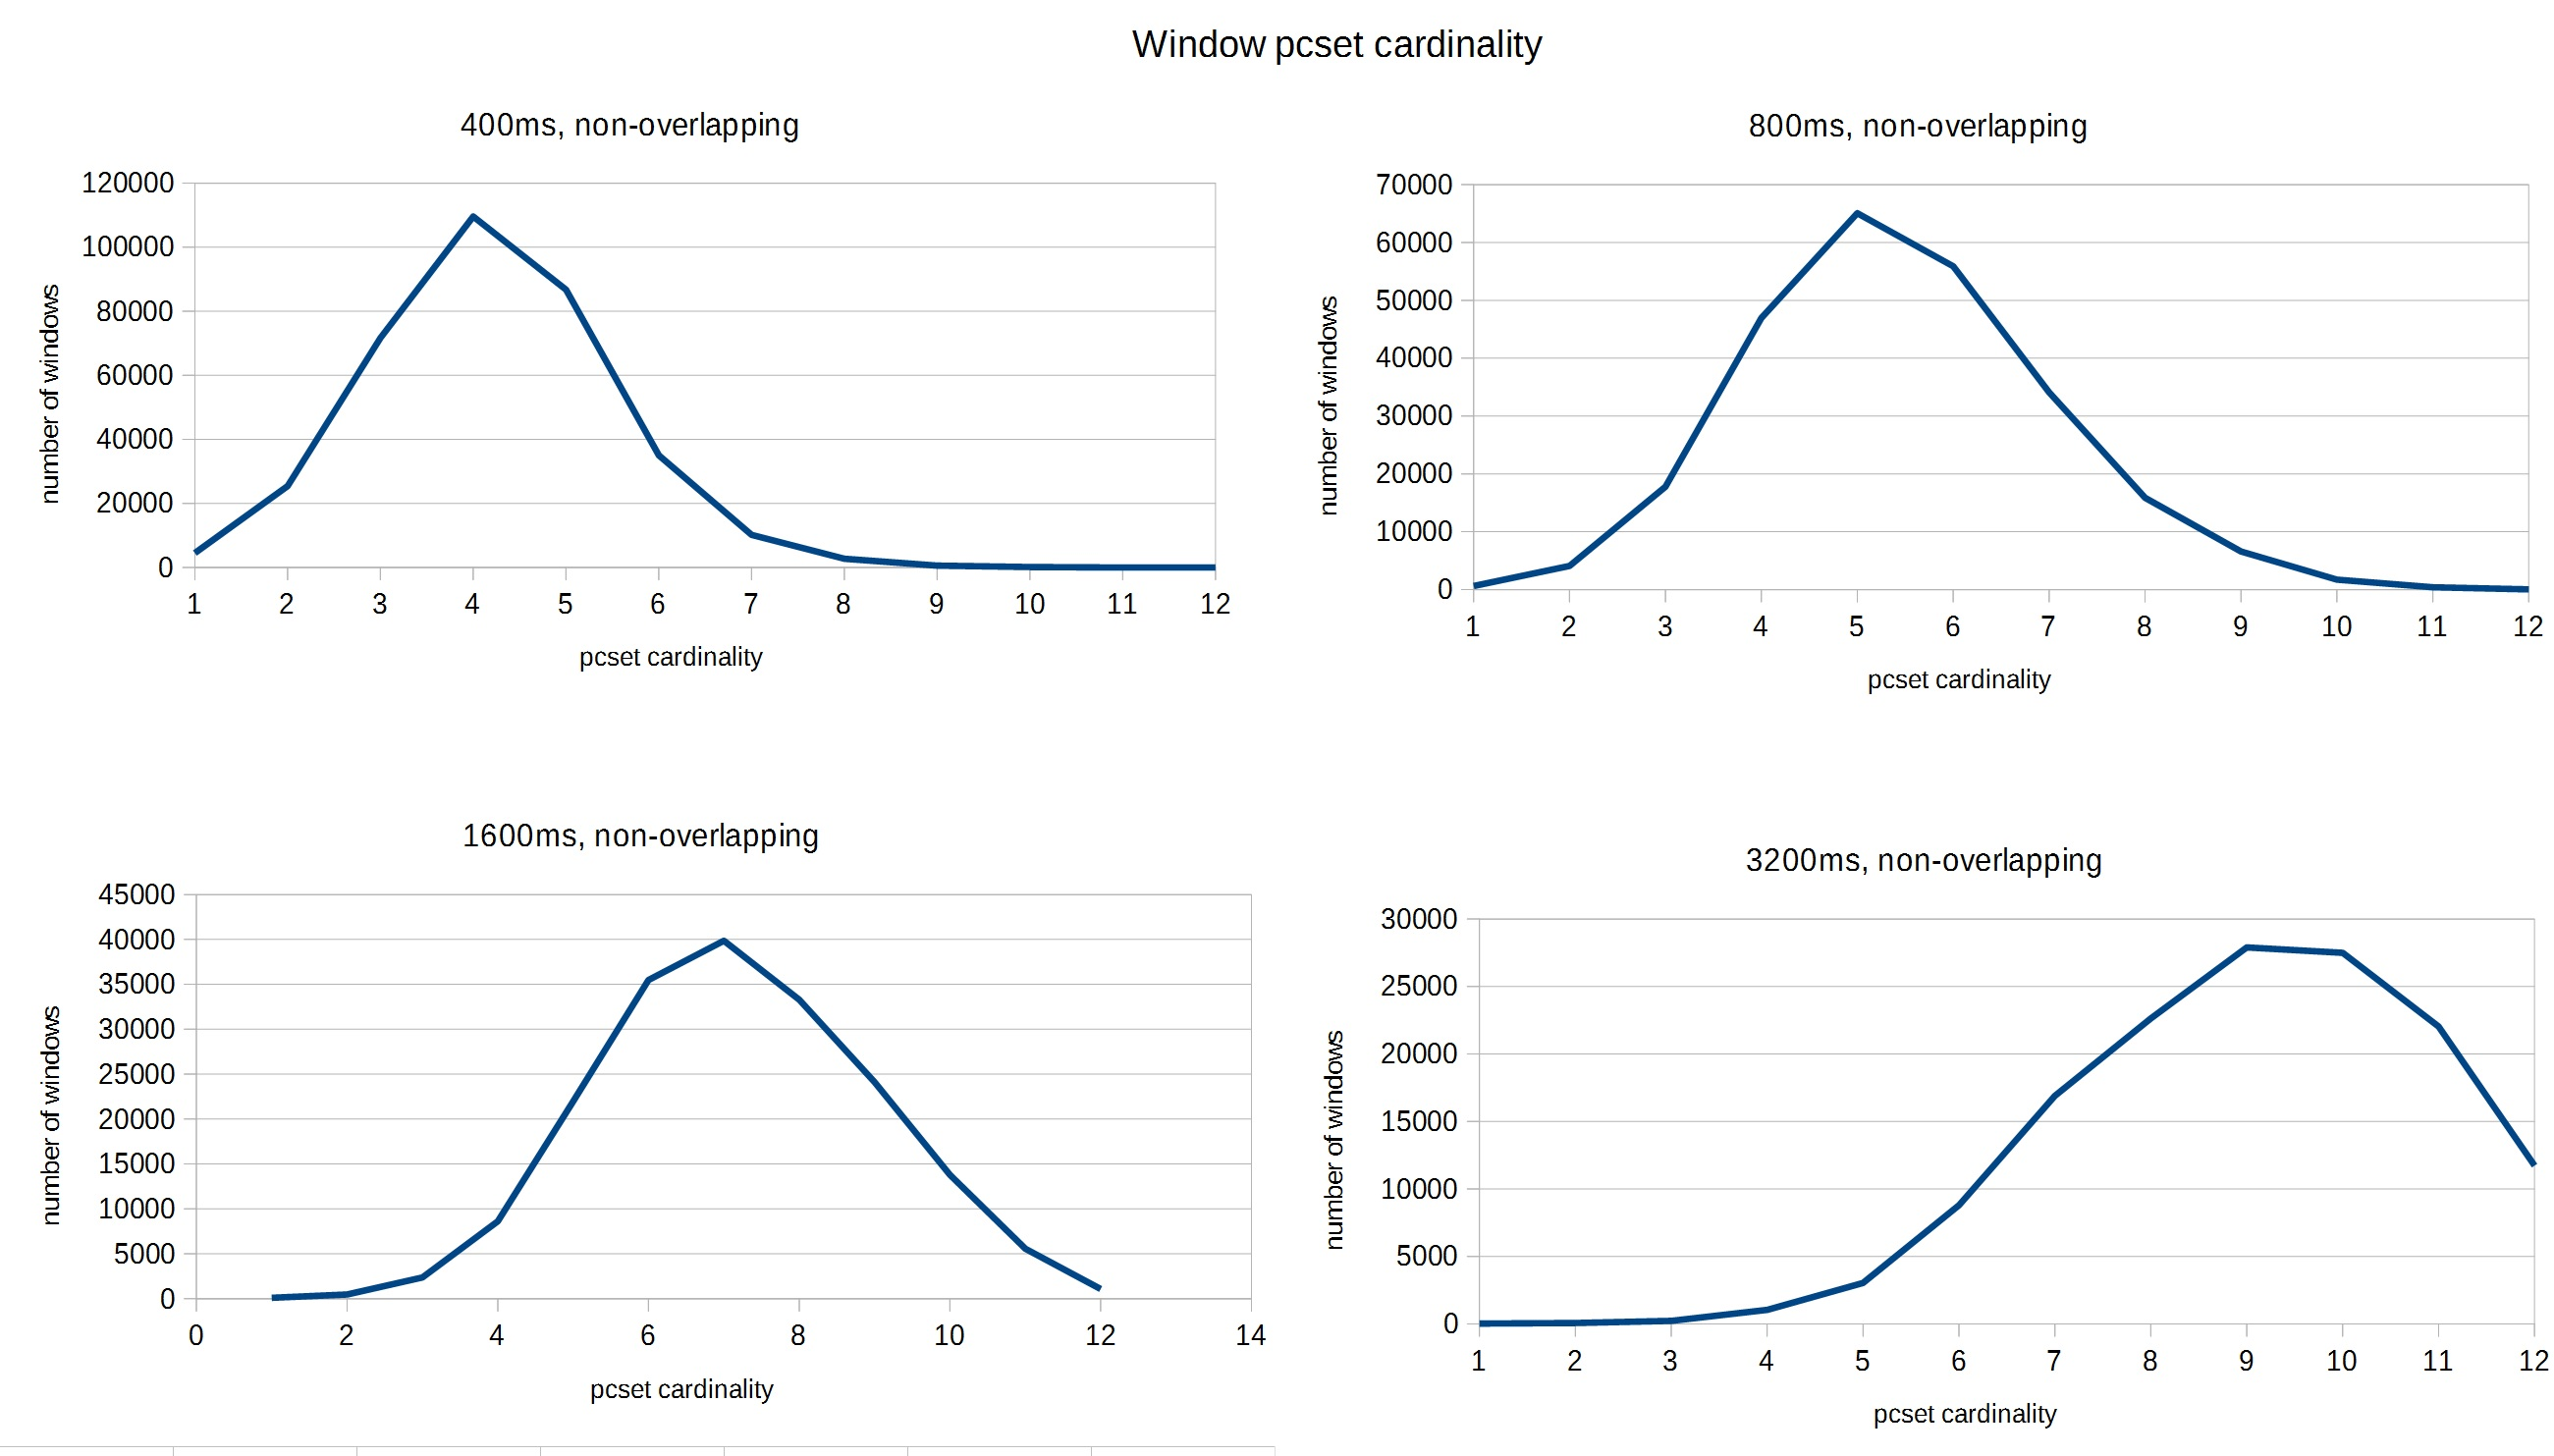
\includegraphics[width=8in]{cardinalities.jpg}
	\caption{Average pc-set cardinalities for four window sizes.  As window size increases, so does average cardinality.}
	\label{cardinalities}
\end{figure}
\end{landscape}

%perplexity and entropy
Perplexity, alongside its information-theoretical partner entropy, can be used to provide a measure of the diversity or disorder of a probability distribution.  A perfectly flat pitch class distribution, which would resemble a horizontal line on Figure~\ref{krumhansl}, corresponds to a high perplexity, where each of the twelve pitch classes would be equally likely to appear -- if asked to guess the pitch class of a particular note in the passage, the distribution would do a pretty (in fact, maximally) poor job.  The distribution for a passage consisting of a single pitch class would have a very low perplexity, indicating that the distribution could predict a particular note in the passage with extremely high certainty; if the passage's pitch-class distribution consisted of $100 \%$ $C$ and $0 \%$ for every other pitch class, it would be maximally ordered and perfectly predictive over the passage.

Key profiles like the Krumhansl-Schmuckler, Aarden-Essen, Temperley-Kostka-Payne, or Bellman-Budge resemble neither case.  These distributions encode information regarding the relative importance of different pitch classes, so their pitch ``guesses" will not be completely random, as they would be in the flat-distribution, high-perplexity case.  But each of these key profiles also encodes non-zero probabilities for all twelve pitch classes, acknowledging that the determination of a passage's key does not preclude the appearance of any member of the aggregate.  Key profiles imply that the pitch-class distributions of tonal music are partially ordered and partially disordered -- not in music theoretical senses of higher/lower pitch, syntax, or voice leading, but in the sense that tonal passages typically contain pitch classes appearing in unequal relative proportions predictable in advance.

The perplexity $PP$ of a probability distribution $p$ may be calculated from its entropy $H(p)$:
\begin{equation}
PP = 2^{H(p)} = 2^{-\sum_{x} p(x) \log_2 p(x)}
\end{equation}
The summation here takes each possible value $x$ (in the pitch-class case, there are 12) and adds up the sum of the value's probability $p(x)$ times the logarithm of its probability $\log_2 p(x)$.  In the flat-distributional case where each of the 12 pitch classes is equally likely, this reduces to the maximum perplexity of a key profile:
\begin{align*}
PP &= 2^{-\big(\frac{1}{12} \log_2 \frac{1}{12} + \frac{1}{12} \log_2 \frac{1}{12} + ...\big)} \\
 &= 2^{-12\big(\frac{1}{12} \log_2 \frac{1}{12}\big)} \\
 &= 2^{-\log_2 \frac{1}{12}} = 2^{\log_2 12} = 12
\end{align*}
Heuristically, perplexity tells us that the model is like the roll of a $PP$-sided die; in the flat-distributional case, predicting a single pitch would be literally equivalent to rolling a fair 12-sided die.  At the other extreme, a minimally-perplexed probability distribution containing a single pitch class with $100\%$ probability has a perplexity of 1 -- its predictions are like rolling a single-sided die.

To match a given passage's pitch-class probability distribution perplexity to that of a key profile, I note that the Bellman-Budge profile yields a perplexity of approximately 8.1 -- similar to that of rolling an 8-sided die.\footnote{Other profiles yield very similar perplexities.  For example, I generated pitch-class profiles for each tune head in the corpus, assembling statistics based on hand-annotated keys in order to produce a ``YJaMP key profile."  The resulting vector hewed fairly closely to Bellmann-Budge (\cite{bellmann2005}), both in terms of its perplexity and the distribution's overall shape.  For code details, see jazzKey.py at \href{github.com/andrewdjones/YJaMP_Analysis}{github.com/andrewdjones/YJaMP\_Analysis}.}  Whichever segmentation window size produces probability distributions with perplexities closest to that value is likely the most appropriate for each recording.  The duration of these windows ranges from a couple of seconds in fast tunes to 30 seconds or more in ballads.

%sliding and cosine optimization
Optimizing the resulting choice of key for each window proceeds in two steps.  First, the key-finding algorithm segments a window of the perplexity-calculated duration and compares its pitch-class distribution to the Bellman-Budge profiles.  I assume that key-to-key variance in profiles is small, so the algorithm sees the same major mode profile and minor mode profile for each possible tonic.  It then choose whichever Bellman-Budge transposition minimizes the cosine distance between it and the window's distribution.  The cosine distance measures the directional alignment of the two twelve-dimensional vectors, discounting their magnitude; this encodes the notion that the absolute frequencies of appearance for pitch classes in the window and profile matter less than their proportional relation to one another.\footnote{Formally, the cosine distance $\cos(\theta)$ between two pitch class vectors $\mathbf{p_1}$ and $\mathbf{p_2}$ is $\cos(\theta) = \frac{\mathbf{p_1} \cdot \mathbf{p_2}}{\| \mathbf{p_1} \| \| \mathbf{p_2} \|}$, the dot product of the vectors divided by the product of their magnitudes.  This approach is similar to but distinct from the Euclidean metric advocated in \cite{albrecht2013}.}  Second, following \cite{wq2017}, the key-finder slides the window through the composition by a small durational increment and re-calculates the best-fit key at each step.

%Sliding, interonsets, and chord temporal stability
Setting this sliding increment impacts both the rate at which the algorithm produces key changes and, more subtly, the ontology in which chords are embedded.  Generally speaking, key assignments change as new pitch classes modify the locally-windowed distribution, and the window sliding increment represents the shortest possible time scale over which the algorithmic agent looks for such changes.  But short-duration, absolute time sliding increments also challenge the temporal stability of chord objects, since the limiting case (say, an increment of 1ms) might well separate pitches we (or an algorithm) might otherwise count as part of the same ``chord" into several different windows.  As a consequence of YJaMP's MIDI encoding, the temporal quantization performed by printed scores never aligns near-simultaneities into exact verticalities -- so the choice of what to call a ``chord" must be made on temporal and distributional grounds.

%Describe inter-onset plot
Figure~\ref{io_plot} plots inter-onset times between the individual pitches of the YJaMP corpus.  Taken directly from the MIDI onset times for each piano key struck, this plot displays how many note-to-note inter-onsets appear in the corpus for a range of possible times stretching from 0ms up to 500ms.  Toward the far right of the figure, an inter-onset time of 450ms indicates a comparatively long gap between two key strikes, while inter-onsets toward the left of the figure indicate nearly simultaneous strikes.  Since the MIDI piano setup loses accuracy below about 5ms, the erratic behavior of the plotted distribution between 0-10ms should be taken with a grain of salt.  At spans above 10ms, however, a relatively smooth distribution emerges, where a very large number of inter-onsets at short times decreases rapidly to a local minimum around 50-60ms.  At durations longer than this scale, the number of inter-onsets displays a slight increase; it only returns to the 50-60ms local minimum around 200ms, after which the long tail tapers off.

I note that this distribution intuitively matches what we might expect from superimposing two separate distributions -- one chi-squared like (for $k=1$), with a maximum at $t=0$ms, and one normal or Gaussian-like, with a mean around $t=130$ms.  The populations represented by the two distributions might then map onto the temporal behavior expected of intra-chord inter-onsets, like fast melodic runs or pitches rolled but struck nearly simultaneously, and inter-chord onsets, as when one roughly simultaneous chord sounds some temporal delay after another.  To posit Figure~\ref{io_plot} as arising from the statistics of two different populations is to enunciate an ontological framing for chords: under such a description, chords consist of sets of pitches struck very close to one another (that is, within about 50ms) which tend to be separated from one another by 50-200ms.  Chords might be thought to ``stabilize," temporally speaking, around 50ms.\footnote{Empiricists and interpreters alike tend to locate the shortest span for human auditory attention in this regime; Justin London and Michel Chion cite 100ms and 40ms, respectively. (\cite{london2012}, p.\ 28; \cite{chion2016}, p.\ 24.)  Note that neither kind of analyst does so on the basis described here.}  As a result, the shortest-duration objects the algorithms of Chapters 3 and 4 tally as ``chords" are the contents of 50ms time windows.

\begin{figure}
	\centering
	\caption{A plot of note inter-onsets versus time for pitches in the YJaMP corpus.  Two types of behavior appear: decreasing counts as time increases, for very short times, and increased counts between 50ms and 200ms.  Below about 5ms, the MIDI piano's accuracy becomes erratic and suspect.}
	\label{io_plot}
	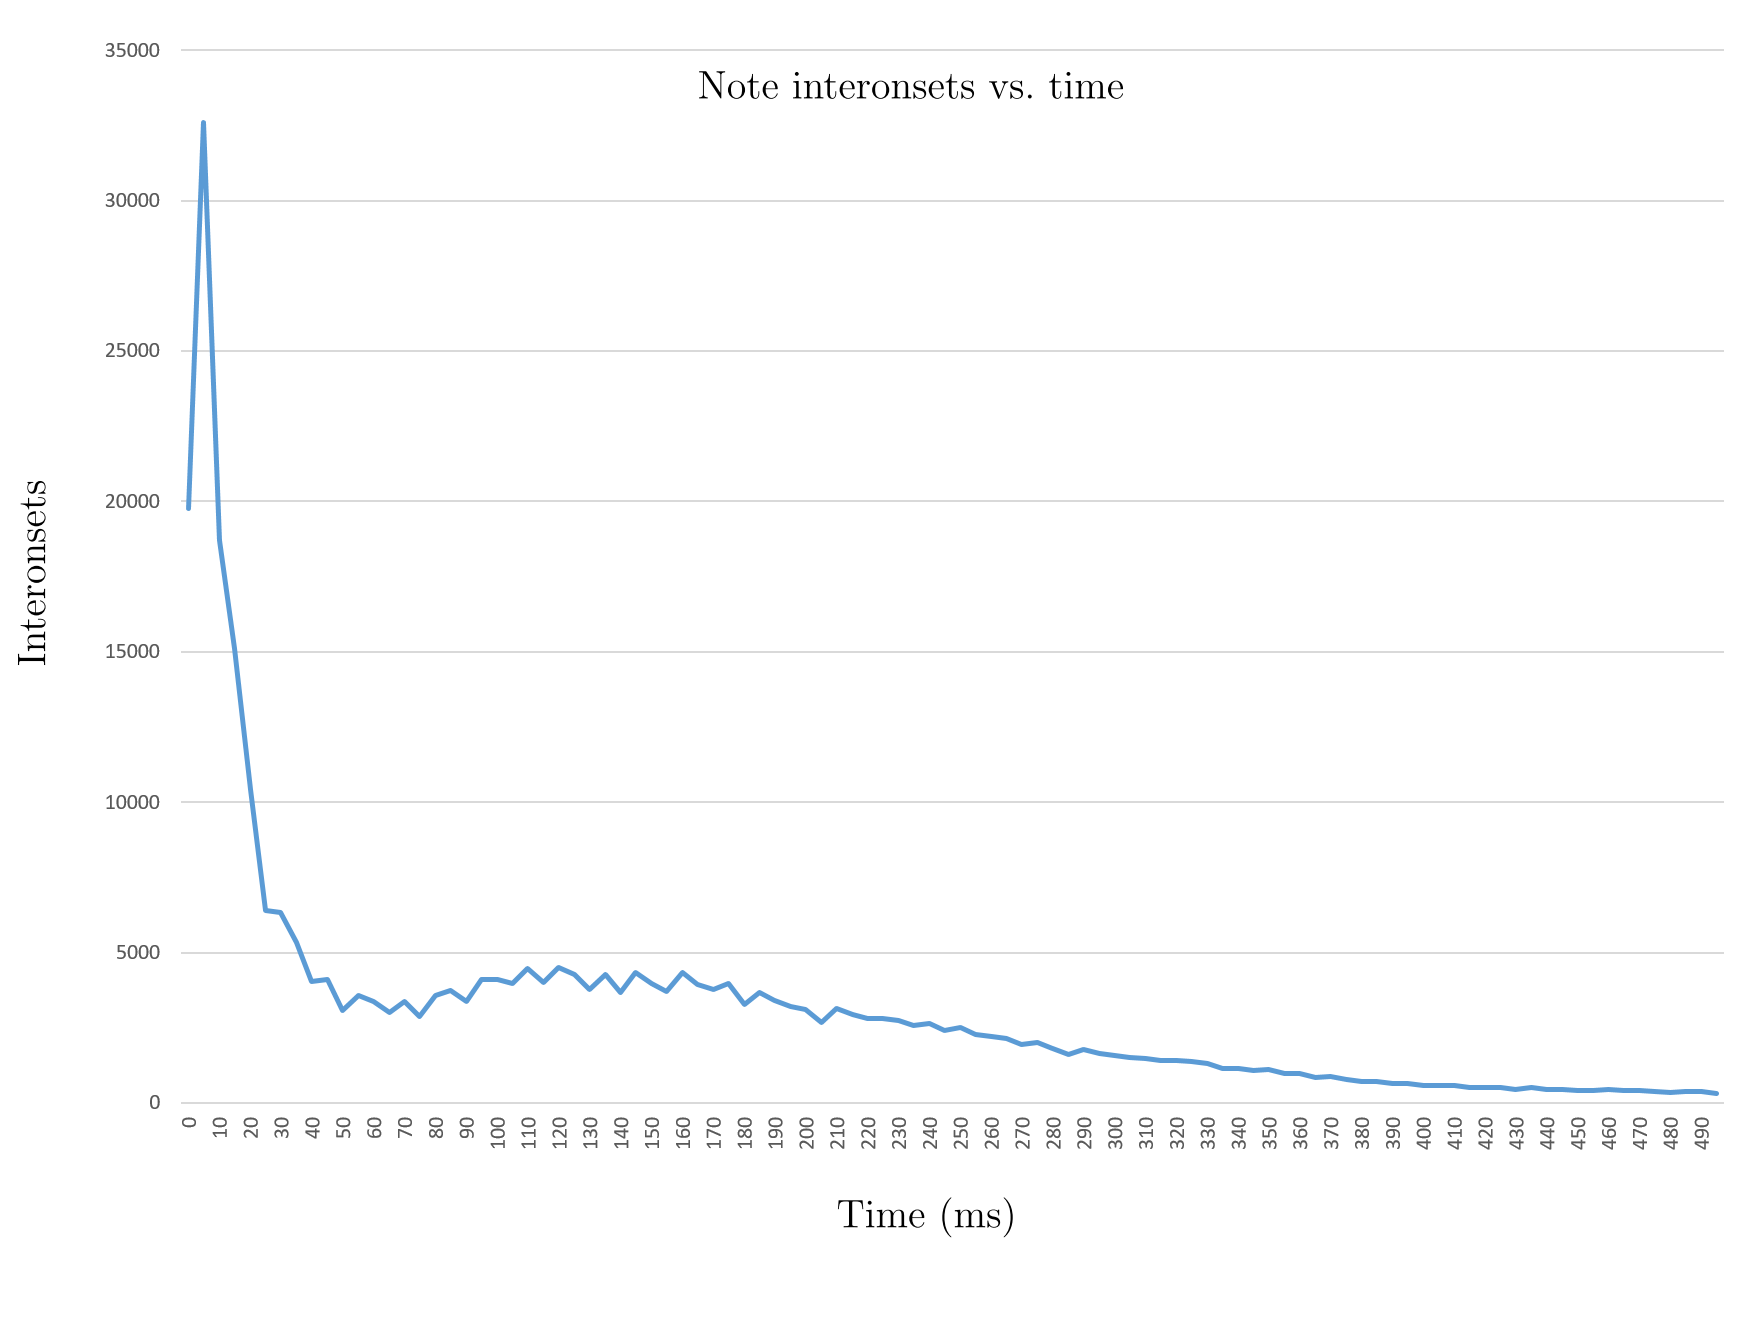
\includegraphics[width=5.9in]{io_plot.png}
\end{figure}

%sliding increment from perplexity change
The status of the 50ms inter-onsets also has ramifications for window perplexity. At very short window sizes (below 50ms), the average perplexity across all windows in a given performance levels out at approximately the average number of pitches sounding at any given moment.  For each recorded track, there is then some slightly larger window size at which the average perplexity begins to increase over this baseline level.  The time scale at which average window perplexity first increases by $30\%$ over its short-duration (ca.\ 50ms) value sets the sliding increment for the segmented windows in the key-finding algorithm.  We might think of this sliding increment, which varies from track to track, as the shortest time scale at which chords might be expected to change at the track's performance tempo. 

%confidence
As a result, each ``chord" in a tune ends up in several possible windows of the same duration.  Since the key-finding algorithm assigns a best-fit key for each window, each chord may have several different possible key assignments.  To disambiguate, the algorithm employs a confidence measure: the degree to which a given key assignment outperforms the model's next-best guess.  Since the predicted key for a window corresponds to the minimum cosine distance ($d_1$) between the window's distribution and the possible key profiles, the model's next-best guess is the key with the second-shortest distance ($d_2$).  One measure for the confidence of the model's guess is then $1 - d_1/d_2$, which approaches 1 when the best guess is very close to the window distribution and the second-best is very far.  If no windows containing a particular chord have confidences higher than $30\%$, I mark the key as ambiguous; otherwise, the key-finder tags the chord with the local key from the window yielding the highest confidence value.

%problematize/ontologize
It is worth asking whether this ``key" assignment really says the same thing as a human-annotated one.  ``Key" in general stands for a complex concept entangling macroharmony and centricity, to borrow Tymozcko's formulation regarding limited pitch class collections with some tonic.\footnote{See \cite{tymoczko2010}, especially Chapters 1 and 5.}  Human listeners or analysts presumably consider voicing, cadence and phrase structure, metric placement, and many other factors when determining a passage's key.  Key-finding algorithms based on pitch-class profiles, however, employ algorithmic agents instead of human ones, and the properties of the resulting key determinations are grounded only in the indexical signs the algorithm uses to make its decisions.  When an algorithmic key-finder of this kind $A_1$ and a human agent $A_2$ both determine that a passage of music ``is in" a particular key, the interpretants refer to objects ($O_1$, $O_2$) with necessarily different semiotic ontologies.  For the algorithm, keys do not have properties like ``indicated by many $ii-V-I$ progressions" or ``signaled by passages ending with a cadence in the tonic" (though pitch-class translation of the former might find indirect support in the passage's pitch class statistics).

I do not claim that each key assigned to a passage by the algorithm corresponds to the kind of key object a human would assign, but rather that the automated key assignments afford certain kinds of indexical inquiry.  If a human analyst assigns a key to a passage by noticing what appears to be a $V-I$ progression, the resulting representation of the data already encodes chord-behavioral assumptions grounded in the way the agent turns signed indices into key interpretants.  This is excellent for the accuracy of key identification, but it introduces potential circularity if the analyst then tries to determine what harmonic progressions occurred in the passage.  When an analyst states that $V-I$ has an important progression status in any given key, the claim reflects both the properties of the key category and the response to indices by which it is observed and assigned.  If an algorithmic agent of the kind above can be made to say that $V-I$ has an important progression status in any given key, the claim rests on a different semiotic structure -- with no \emph{a priori} knowledge about what kinds of progression index a key, key profile-tagged corpora can provide an important ground for claims regarding tonal syntactic progressions.

%set up transposition to scale degree sets
With these keys in hand, chapters 3 and 4 pursue inquiry of this type.  To isolate syntactic progressions relative to some local key, the key-finding algorithm assigns keys to each chord in the music and converts all pitch-class sets into local, chromatic \emph{scale-degree sets}.  Each scale-degree set consists of the semitonal pitch-class set data transposed relative to the local key.  Relative to the local tonic (set as chromatic scale degree 0), Table~\ref{sds} shows the most frequent scale-degree sets of cardinality 4 or greater found in YJaMP.

\begin{table}
\caption{The most common locally-transposed scale-degree sets in the YJaMP corpus with cardinalities larger than 3.}
  \centering
\begin{tabular}{l | l | l}
\hline\hline
Scale-degree set & Counts & Potential interpretation \\ [0.5ex]
\hline
$[0, 4, 7, 11]$ &	2783	& $I^7$ \\
$[0, 4, 5, 9]$ &	2217	& $IV^7$\\
$[2, 4, 7, 11]$ &	2110	& $iii^7$\\
$[0, 2, 4, 7]$ &	1924	&\\
$[0, 2, 5, 7]$ &	1878	&\\
$[0, 3, 7, 8]$ &	1804	& $\flat VI^7$\\
$[0, 4, 7, 9]$ &	1712	& $vi^7$\\
$[0, 2, 5, 9]$ &	1659	& $ii^7$\\
$[0, 5, 7, 9]$ &	1253	&\\
$[0, 3, 5, 7]$ &	1252	&\\
$[0, 2, 7, 9]$ &	1238	&\\
$[0, 2, 4, 7, 11]$ &	1165 &	$I^9$\\
$[0, 2, 7, 8]$ &	1128	&\\
$[0, 2, 7, 11]$ &	1114	&\\
$[2, 5, 7, 11]$ &	1105	& $V^7$\\
$[0, 4, 5, 7, 9]$ &	1093	& $IV^9$\\
$[2, 4, 7, 9]$ &	1055	&\\
$[2, 7, 9, 11]$ &	1009	& $V$ add \nth{9}\\[1ex]	 
\hline
\end{tabular}
\label{sds}
\end{table}

This seemingly-unremarkable list makes no assumptions about chord structure, consonance, or voice-leading.  Dissonant clusters are treated exactly the same as stacks of perfect fifths, pentatonic scales, and seventh chords.  No reduction of non-harmonic tones has been employed.  Nevertheless, scale-degree sets corresponding to $I^7$, the local tonic, constitute the most frequent four-note scale-degree sets in the corpus, and minor, major, and dominant seventh chords on scale degrees strongly predicted by traditional syntactic theories all appear high on the list.  As these chords were not known to the algorithmic agent making the key assignments, we might take their appearance here as confirmation that human analysts are right to connect chord progressions and keys.  Chapter 3 uses $ii$ chords to introduce methods for examining the temporal progression properties of scale-degree sets, and Chapter 4 provides methods for grouping scale-degree sets into categories based on similarities in their progression statistics.  Both of these modes of analysis rest on the particular nature of these scale-degree sets -- this particular method of turning the YJaMP recordings into harmonic objects.  Just as the first half of this chapter used algorithmically-produced voicing objects to both complicate and lend support to jazz theoretical interpretants, the following chapters will treat scale-degree set objects as signed indices in an attempt to reproduce and expand traditional statements regarding syntactic progressions.  Many object-ifications of a performance corpus are possible, but the one presented here affords a particular alignment between computational semiotic processes and human-analytical ones.
	
